\documentclass[twoside]{book}

% Packages required by doxygen
\usepackage{fixltx2e}
\usepackage{calc}
\usepackage{doxygen}
\usepackage[export]{adjustbox} % also loads graphicx
\usepackage{graphicx}
\usepackage[utf8]{inputenc}
\usepackage{makeidx}
\usepackage{multicol}
\usepackage{multirow}
\PassOptionsToPackage{warn}{textcomp}
\usepackage{textcomp}
\usepackage[nointegrals]{wasysym}
\usepackage[table]{xcolor}

% Font selection
\usepackage[T1]{fontenc}
\usepackage[scaled=.90]{helvet}
\usepackage{courier}
\usepackage{amssymb}
\usepackage{sectsty}
\renewcommand{\familydefault}{\sfdefault}
\allsectionsfont{%
  \fontseries{bc}\selectfont%
  \color{darkgray}%
}
\renewcommand{\DoxyLabelFont}{%
  \fontseries{bc}\selectfont%
  \color{darkgray}%
}
\newcommand{\+}{\discretionary{\mbox{\scriptsize$\hookleftarrow$}}{}{}}

% Page & text layout
\usepackage{geometry}
\geometry{%
  a4paper,%
  top=2.5cm,%
  bottom=2.5cm,%
  left=2.5cm,%
  right=2.5cm%
}
\tolerance=750
\hfuzz=15pt
\hbadness=750
\setlength{\emergencystretch}{15pt}
\setlength{\parindent}{0cm}
\setlength{\parskip}{3ex plus 2ex minus 2ex}
\makeatletter
\renewcommand{\paragraph}{%
  \@startsection{paragraph}{4}{0ex}{-1.0ex}{1.0ex}{%
    \normalfont\normalsize\bfseries\SS@parafont%
  }%
}
\renewcommand{\subparagraph}{%
  \@startsection{subparagraph}{5}{0ex}{-1.0ex}{1.0ex}{%
    \normalfont\normalsize\bfseries\SS@subparafont%
  }%
}
\makeatother

% Headers & footers
\usepackage{fancyhdr}
\pagestyle{fancyplain}
\fancyhead[LE]{\fancyplain{}{\bfseries\thepage}}
\fancyhead[CE]{\fancyplain{}{}}
\fancyhead[RE]{\fancyplain{}{\bfseries\leftmark}}
\fancyhead[LO]{\fancyplain{}{\bfseries\rightmark}}
\fancyhead[CO]{\fancyplain{}{}}
\fancyhead[RO]{\fancyplain{}{\bfseries\thepage}}
\fancyfoot[LE]{\fancyplain{}{}}
\fancyfoot[CE]{\fancyplain{}{}}
\fancyfoot[RE]{\fancyplain{}{\bfseries\scriptsize Generated by Doxygen }}
\fancyfoot[LO]{\fancyplain{}{\bfseries\scriptsize Generated by Doxygen }}
\fancyfoot[CO]{\fancyplain{}{}}
\fancyfoot[RO]{\fancyplain{}{}}
\renewcommand{\footrulewidth}{0.4pt}
\renewcommand{\chaptermark}[1]{%
  \markboth{#1}{}%
}
\renewcommand{\sectionmark}[1]{%
  \markright{\thesection\ #1}%
}

% Indices & bibliography
\usepackage{natbib}
\usepackage[titles]{tocloft}
\setcounter{tocdepth}{3}
\setcounter{secnumdepth}{5}
\makeindex

% Hyperlinks (required, but should be loaded last)
\usepackage{ifpdf}
\ifpdf
  \usepackage[pdftex,pagebackref=true]{hyperref}
\else
  \usepackage[ps2pdf,pagebackref=true]{hyperref}
\fi
\hypersetup{%
  colorlinks=true,%
  linkcolor=blue,%
  citecolor=blue,%
  unicode%
}

% Custom commands
\newcommand{\clearemptydoublepage}{%
  \newpage{\pagestyle{empty}\cleardoublepage}%
}

\usepackage{caption}
\captionsetup{labelsep=space,justification=centering,font={bf},singlelinecheck=off,skip=4pt,position=top}

%===== C O N T E N T S =====

\begin{document}

% Titlepage & ToC
\hypersetup{pageanchor=false,
             bookmarksnumbered=true,
             pdfencoding=unicode
            }
\pagenumbering{alph}
\begin{titlepage}
\vspace*{7cm}
\begin{center}%
{\Large My Project }\\
\vspace*{1cm}
{\large Generated by Doxygen 1.8.13}\\
\end{center}
\end{titlepage}
\clearemptydoublepage
\pagenumbering{roman}
\tableofcontents
\clearemptydoublepage
\pagenumbering{arabic}
\hypersetup{pageanchor=true}

%--- Begin generated contents ---
\chapter{Todo List}
\label{todo}
\Hypertarget{todo}

\begin{DoxyRefList}
\item[\label{todo__todo000001}%
\Hypertarget{todo__todo000001}%
Member \hyperlink{class_d_box_a60558669bcb1b761aab592c0d70b64ce}{D\+Box\+:\+:mod} (const \hyperlink{class_point}{Point} \&a\+\_\+pt) const]Determine the purpose of this function 
\end{DoxyRefList}
\chapter{Hierarchical Index}
\section{Class Hierarchy}
This inheritance list is sorted roughly, but not completely, alphabetically\+:\begin{DoxyCompactList}
\item \contentsline{section}{Auto\+Start}{\pageref{class_auto_start}}{}
\item \contentsline{section}{Auto\+Start\+Leaf}{\pageref{class_auto_start_leaf}}{}
\item \contentsline{section}{Conv\+Kernel}{\pageref{class_conv_kernel}}{}
\begin{DoxyCompactList}
\item \contentsline{section}{Cutoff\+Kernel}{\pageref{class_cutoff_kernel}}{}
\end{DoxyCompactList}
\item \contentsline{section}{D\+Box}{\pageref{class_d_box}}{}
\item \contentsline{section}{DX}{\pageref{class_d_x}}{}
\item \contentsline{section}{elem}{\pageref{structelem}}{}
\item \contentsline{section}{F\+F\+T1D}{\pageref{class_f_f_t1_d}}{}
\begin{DoxyCompactList}
\item \contentsline{section}{F\+F\+T1\+DW}{\pageref{class_f_f_t1_d_w}}{}
\end{DoxyCompactList}
\item \contentsline{section}{F\+F\+T\+MD}{\pageref{class_f_f_t_m_d}}{}
\item \contentsline{section}{Hockney}{\pageref{class_hockney}}{}
\item \contentsline{section}{Particle}{\pageref{class_particle}}{}
\item \contentsline{section}{Particle\+Set}{\pageref{class_particle_set}}{}
\item \contentsline{section}{Particle\+Shift}{\pageref{class_particle_shift}}{}
\item \contentsline{section}{Particle\+Velocities}{\pageref{class_particle_velocities}}{}
\item \contentsline{section}{Point}{\pageref{class_point}}{}
\item \contentsline{section}{Rect\+M\+D\+Array$<$ T, C $>$}{\pageref{class_rect_m_d_array}}{}
\item \contentsline{section}{R\+K4$<$ X, F, dX $>$}{\pageref{class_r_k4}}{}
\item \contentsline{section}{Trace\+Timer}{\pageref{class_trace_timer}}{}
\end{DoxyCompactList}

\chapter{Class Index}
\section{Class List}
Here are the classes, structs, unions and interfaces with brief descriptions\+:\begin{DoxyCompactList}
\item\contentsline{section}{\hyperlink{class_auto_start}{Auto\+Start} }{\pageref{class_auto_start}}{}
\item\contentsline{section}{\hyperlink{class_auto_start_leaf}{Auto\+Start\+Leaf} }{\pageref{class_auto_start_leaf}}{}
\item\contentsline{section}{\hyperlink{class_conv_kernel}{Conv\+Kernel} }{\pageref{class_conv_kernel}}{}
\item\contentsline{section}{\hyperlink{class_cutoff_kernel}{Cutoff\+Kernel} }{\pageref{class_cutoff_kernel}}{}
\item\contentsline{section}{\hyperlink{class_d_box}{D\+Box} \\*An interval in D\+IM dimensional space }{\pageref{class_d_box}}{}
\item\contentsline{section}{\hyperlink{class_d_x}{DX} \\*Class representing the increment of a single point }{\pageref{class_d_x}}{}
\item\contentsline{section}{\hyperlink{structelem}{elem} }{\pageref{structelem}}{}
\item\contentsline{section}{\hyperlink{class_f_f_t1_d}{F\+F\+T1D} }{\pageref{class_f_f_t1_d}}{}
\item\contentsline{section}{\hyperlink{class_f_f_t1_d_w}{F\+F\+T1\+DW} }{\pageref{class_f_f_t1_d_w}}{}
\item\contentsline{section}{\hyperlink{class_f_f_t_m_d}{F\+F\+T\+MD} }{\pageref{class_f_f_t_m_d}}{}
\item\contentsline{section}{\hyperlink{class_hockney}{Hockney} }{\pageref{class_hockney}}{}
\item\contentsline{section}{\hyperlink{class_particle}{Particle} \\*Represents a single particle in a \hyperlink{class_particle_set}{Particle\+Set} }{\pageref{class_particle}}{}
\item\contentsline{section}{\hyperlink{class_particle_set}{Particle\+Set} \\*Represents a collection of particles, conforming to the X class in \hyperlink{class_r_k4}{R\+K4}. Also contains the persistent data required to compute the right-\/hand side in Particles\+Velocities }{\pageref{class_particle_set}}{}
\item\contentsline{section}{\hyperlink{class_particle_shift}{Particle\+Shift} \\*Represents an increment in a \hyperlink{class_particle_set}{Particle\+Set} conforming to the dX class in \hyperlink{class_r_k4}{R\+K4} }{\pageref{class_particle_shift}}{}
\item\contentsline{section}{\hyperlink{class_particle_velocities}{Particle\+Velocities} \\*Class for computing the R\+HS in \hyperlink{class_r_k4}{R\+K4}, corresponding to the template parameter F }{\pageref{class_particle_velocities}}{}
\item\contentsline{section}{\hyperlink{class_point}{Point} \\*A point in space }{\pageref{class_point}}{}
\item\contentsline{section}{\hyperlink{class_rect_m_d_array}{Rect\+M\+D\+Array$<$ T, C $>$} }{\pageref{class_rect_m_d_array}}{}
\item\contentsline{section}{\hyperlink{class_r_k4}{R\+K4$<$ X, F, d\+X $>$} \\*Generic explicit \hyperlink{class_r_k4}{R\+K4} algorithm }{\pageref{class_r_k4}}{}
\item\contentsline{section}{\hyperlink{class_trace_timer}{Trace\+Timer} }{\pageref{class_trace_timer}}{}
\end{DoxyCompactList}

\chapter{Class Documentation}
\hypertarget{class_auto_start}{}\section{Auto\+Start Class Reference}
\label{class_auto_start}\index{Auto\+Start@{Auto\+Start}}
\subsection*{Public Member Functions}
\begin{DoxyCompactItemize}
\item 
\mbox{\Hypertarget{class_auto_start_a9e0816a258371fe0ec3ea3c14267ef5c}\label{class_auto_start_a9e0816a258371fe0ec3ea3c14267ef5c}} 
{\bfseries Auto\+Start} (\hyperlink{class_trace_timer}{Trace\+Timer} $\ast$a\+\_\+timer, char $\ast$mutex, char $\ast$child\+Mutex)
\item 
\mbox{\Hypertarget{class_auto_start_aa3bd9f51f4f29c99c2147903cc6db7d2}\label{class_auto_start_aa3bd9f51f4f29c99c2147903cc6db7d2}} 
{\bfseries Auto\+Start} (\hyperlink{class_trace_timer}{Trace\+Timer} $\ast$a\+\_\+timer, char $\ast$mutex)
\item 
\mbox{\Hypertarget{class_auto_start_a391135bddc96b9bda90d46711329fb29}\label{class_auto_start_a391135bddc96b9bda90d46711329fb29}} 
bool {\bfseries active} ()
\end{DoxyCompactItemize}


The documentation for this class was generated from the following files\+:\begin{DoxyCompactItemize}
\item 
utils/timer/C\+H\+\_\+\+Timer.\+H\item 
utils/timer/C\+H\+\_\+\+Timer.\+cpp\end{DoxyCompactItemize}

\hypertarget{class_auto_start_leaf}{}\section{Auto\+Start\+Leaf Class Reference}
\label{class_auto_start_leaf}\index{Auto\+Start\+Leaf@{Auto\+Start\+Leaf}}
\subsection*{Public Member Functions}
\begin{DoxyCompactItemize}
\item 
\mbox{\Hypertarget{class_auto_start_leaf_ad31126dbec37c0245fd08bb77be1612b}\label{class_auto_start_leaf_ad31126dbec37c0245fd08bb77be1612b}} 
{\bfseries Auto\+Start\+Leaf} (\hyperlink{class_trace_timer}{Trace\+Timer} $\ast$a\+\_\+timer)
\item 
\mbox{\Hypertarget{class_auto_start_leaf_ac6ebea5f14cfea49095514d89f107691}\label{class_auto_start_leaf_ac6ebea5f14cfea49095514d89f107691}} 
bool {\bfseries active} ()
\end{DoxyCompactItemize}


The documentation for this class was generated from the following files\+:\begin{DoxyCompactItemize}
\item 
utils/timer/C\+H\+\_\+\+Timer.\+H\item 
utils/timer/C\+H\+\_\+\+Timer.\+cpp\end{DoxyCompactItemize}

\hypertarget{class_conv_kernel}{}\section{Conv\+Kernel Class Reference}
\label{class_conv_kernel}\index{Conv\+Kernel@{Conv\+Kernel}}
Inheritance diagram for Conv\+Kernel\+:\begin{figure}[H]
\begin{center}
\leavevmode
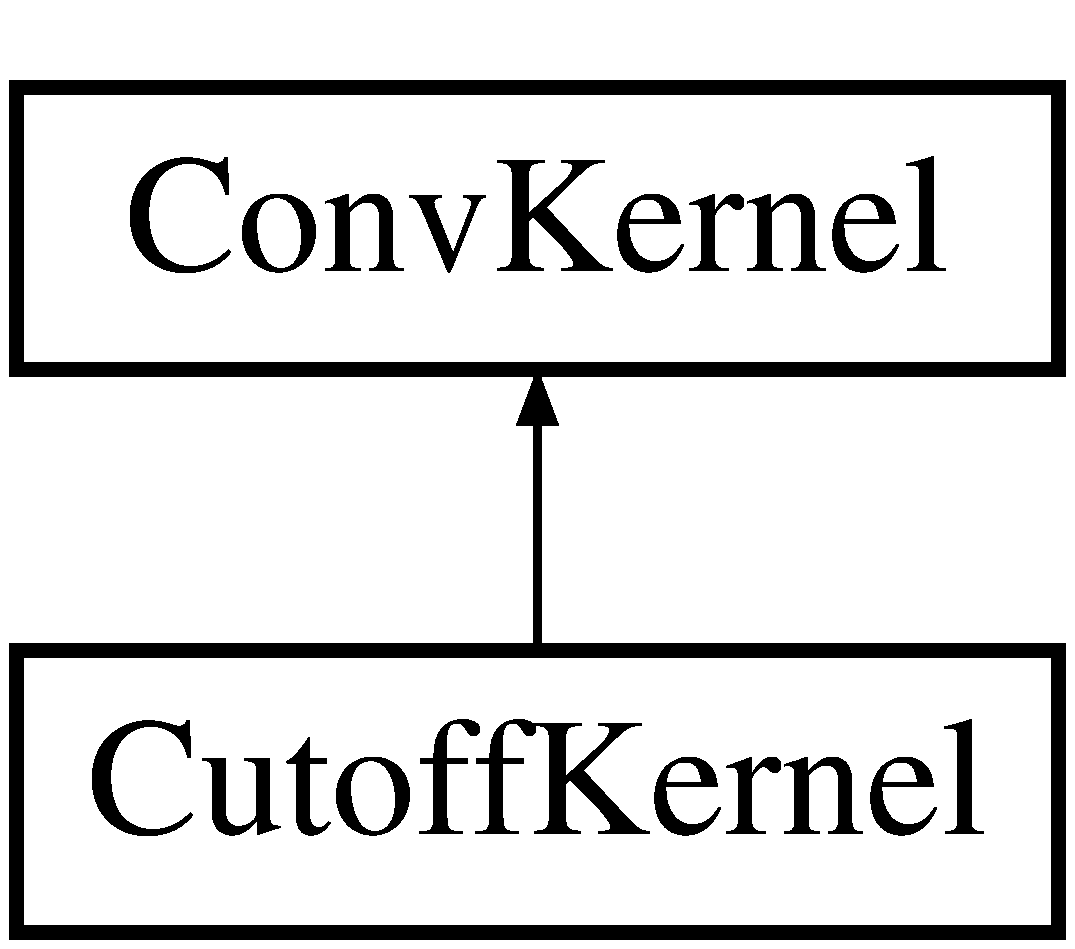
\includegraphics[height=2.000000cm]{class_conv_kernel}
\end{center}
\end{figure}
\subsection*{Public Member Functions}
\begin{DoxyCompactItemize}
\item 
\mbox{\Hypertarget{class_conv_kernel_ab248f15217152f184686de1d0f2e198b}\label{class_conv_kernel_ab248f15217152f184686de1d0f2e198b}} 
\hyperlink{class_conv_kernel_ab248f15217152f184686de1d0f2e198b}{Conv\+Kernel} ()
\begin{DoxyCompactList}\small\item\em Default constructor. \end{DoxyCompactList}\item 
\mbox{\Hypertarget{class_conv_kernel_ac89fb6a91e458daab100910405be97f3}\label{class_conv_kernel_ac89fb6a91e458daab100910405be97f3}} 
virtual \hyperlink{class_conv_kernel_ac89fb6a91e458daab100910405be97f3}{$\sim$\+Conv\+Kernel} ()
\begin{DoxyCompactList}\small\item\em Destructor. \end{DoxyCompactList}\item 
\mbox{\Hypertarget{class_conv_kernel_a97d8ad0d7784ba0861c1dcd72bab1f80}\label{class_conv_kernel_a97d8ad0d7784ba0861c1dcd72bab1f80}} 
virtual void \hyperlink{class_conv_kernel_a97d8ad0d7784ba0861c1dcd72bab1f80}{get\+Kernel} (\hyperlink{class_rect_m_d_array}{Rect\+M\+D\+Array}$<$ complex$<$ double $>$ $>$ \&a\+\_\+src\+Array, double \&a\+\_\+h)=0
\begin{DoxyCompactList}\small\item\em Defines a default-\/constructed \hyperlink{class_rect_m_d_array}{Rect\+M\+D\+Array}. \end{DoxyCompactList}\end{DoxyCompactItemize}


The documentation for this class was generated from the following file\+:\begin{DoxyCompactItemize}
\item 
src/\+Hockney/Conv\+Kernel.\+H\end{DoxyCompactItemize}

\hypertarget{class_cutoff_kernel}{}\section{Cutoff\+Kernel Class Reference}
\label{class_cutoff_kernel}\index{Cutoff\+Kernel@{Cutoff\+Kernel}}
Inheritance diagram for Cutoff\+Kernel\+:\begin{figure}[H]
\begin{center}
\leavevmode
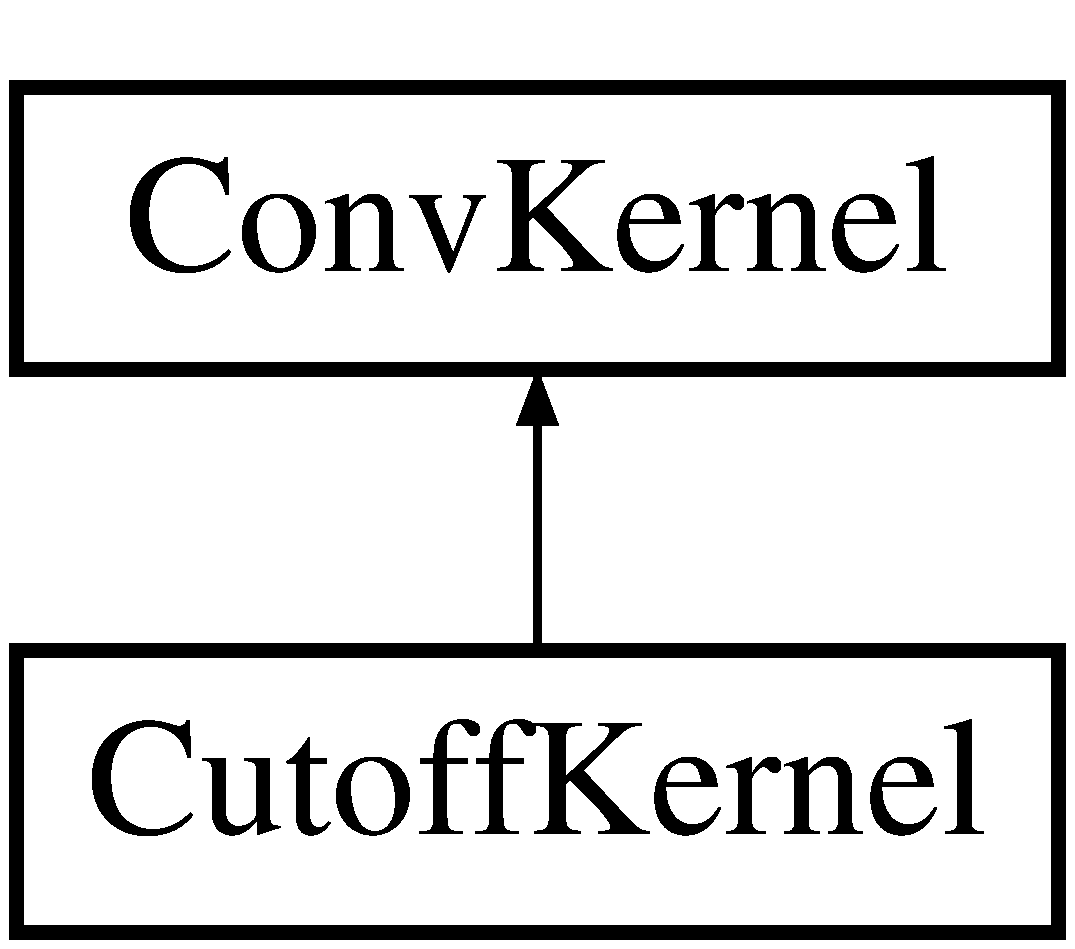
\includegraphics[height=2.000000cm]{class_cutoff_kernel}
\end{center}
\end{figure}
\subsection*{Public Member Functions}
\begin{DoxyCompactItemize}
\item 
\mbox{\Hypertarget{class_cutoff_kernel_a48c10b9caddf5456baef4da2e315d6e6}\label{class_cutoff_kernel_a48c10b9caddf5456baef4da2e315d6e6}} 
{\bfseries Cutoff\+Kernel} (double \&a\+\_\+h, double a\+\_\+delta)
\item 
\mbox{\Hypertarget{class_cutoff_kernel_a9d3c6da0861bc97f3c9d885ecab28489}\label{class_cutoff_kernel_a9d3c6da0861bc97f3c9d885ecab28489}} 
virtual void \hyperlink{class_cutoff_kernel_a9d3c6da0861bc97f3c9d885ecab28489}{get\+Kernel} (\hyperlink{class_rect_m_d_array}{Rect\+M\+D\+Array}$<$ complex$<$ double $>$ $>$ \&a\+\_\+ker\+Array, double \&a\+\_\+h)
\begin{DoxyCompactList}\small\item\em Defines a default-\/constructed \hyperlink{class_rect_m_d_array}{Rect\+M\+D\+Array}. \end{DoxyCompactList}\end{DoxyCompactItemize}


The documentation for this class was generated from the following file\+:\begin{DoxyCompactItemize}
\item 
src/\+Hockney/Cutoff\+Kernel.\+H\end{DoxyCompactItemize}

\hypertarget{class_d_box}{}\section{D\+Box Class Reference}
\label{class_d_box}\index{D\+Box@{D\+Box}}


An interval in D\+IM dimensional space.  




{\ttfamily \#include $<$D\+Box.\+H$>$}

\subsection*{Public Member Functions}
\begin{DoxyCompactItemize}
\item 
\hyperlink{class_d_box_a8a8c5c7cf3bbfee6ecd3372ced15a540}{D\+Box} ()
\begin{DoxyCompactList}\small\item\em Default constructor. \end{DoxyCompactList}\item 
\mbox{\Hypertarget{class_d_box_a5e18be35e68713b75e3b938e1d7929fd}\label{class_d_box_a5e18be35e68713b75e3b938e1d7929fd}} 
\hyperlink{class_d_box_a5e18be35e68713b75e3b938e1d7929fd}{D\+Box} (const \hyperlink{class_point}{Point} \&a\+\_\+low\+Corner, const \hyperlink{class_point}{Point} \&a\+\_\+high\+Corner)
\begin{DoxyCompactList}\small\item\em Constructor for nontrivial \hyperlink{class_d_box}{D\+Box} using two Points. \end{DoxyCompactList}\item 
\mbox{\Hypertarget{class_d_box_a1b1fa391c33d6fed5f6b0766dc64190b}\label{class_d_box_a1b1fa391c33d6fed5f6b0766dc64190b}} 
\hyperlink{class_d_box_a1b1fa391c33d6fed5f6b0766dc64190b}{D\+Box} (const \hyperlink{class_d_box}{D\+Box} \&a\+\_\+\+D\+Box)
\begin{DoxyCompactList}\small\item\em Copy constructor. \end{DoxyCompactList}\item 
\hyperlink{class_d_box}{D\+Box} \hyperlink{class_d_box_a80e097ac4ec5b019d138e07f2d5c22a3}{operator \&} (const \hyperlink{class_d_box}{D\+Box} \&a\+\_\+right\+D\+Box) const
\begin{DoxyCompactList}\small\item\em Computes the intersection of the \hyperlink{class_d_box}{D\+Box} with a\+\_\+right\+D\+Box. \hyperlink{class_d_box}{D\+Box} A\+ND operation. \end{DoxyCompactList}\item 
void \hyperlink{class_d_box_a98da582f742e5e82bdbb740533cc959b}{operator \&=} (const \hyperlink{class_d_box}{D\+Box} \&a\+\_\+right\+D\+Box)
\begin{DoxyCompactList}\small\item\em Computes intersection of \hyperlink{class_d_box}{D\+Box} and a\+\_\+right\+D\+Box in place. \end{DoxyCompactList}\item 
\hyperlink{class_d_box}{D\+Box} \hyperlink{class_d_box_a62403e537be588d0af273cb9d84e089c}{shift} (int a\+\_\+direction, int a\+\_\+offset) const
\begin{DoxyCompactList}\small\item\em Computes shifted \hyperlink{class_d_box}{D\+Box} by a\+\_\+offset in direction a\+\_\+direction. \end{DoxyCompactList}\item 
\hyperlink{class_d_box}{D\+Box} \hyperlink{class_d_box_ad01e33bf0839296a79a315c4dc17f97c}{shift} (const \hyperlink{class_point}{Point} \&a\+\_\+pt) const
\begin{DoxyCompactList}\small\item\em Computes a \hyperlink{class_d_box}{D\+Box} shifted according to the vector a\+\_\+pt. \end{DoxyCompactList}\item 
\hyperlink{class_d_box}{D\+Box} \hyperlink{class_d_box_a390a8b999c556c217cb1f0297691180a}{grow} (int a\+\_\+numpoints) const
\begin{DoxyCompactList}\small\item\em Grow in all of the coordinate directions by a\+\_\+numpoints. \end{DoxyCompactList}\item 
\hyperlink{class_d_box}{D\+Box} \hyperlink{class_d_box_aa764549d6adab28f06409cd769c6b07e}{grow} (const \hyperlink{class_point}{Point} \&a\+\_\+pt) const
\begin{DoxyCompactList}\small\item\em Grow in each coordinate direction by an amount given by the component of a\+\_\+pt. \end{DoxyCompactList}\item 
\hyperlink{class_d_box}{D\+Box} \hyperlink{class_d_box_a0c5ff6539cfad2c35554507a4094a663}{coarsen} (int a\+\_\+numpoints) const
\begin{DoxyCompactList}\small\item\em coarsen in all of the coordinate directions by a\+\_\+numpoints. \end{DoxyCompactList}\item 
\hyperlink{class_d_box}{D\+Box} \hyperlink{class_d_box_aa8b06b12dfb6853ea4a84d03339969dc}{coarsen} (const \hyperlink{class_point}{Point} \&a\+\_\+pt) const
\begin{DoxyCompactList}\small\item\em coarsen in each coordinate direction by an amount given by the component of a\+\_\+pt. \end{DoxyCompactList}\item 
\hyperlink{class_d_box}{D\+Box} \hyperlink{class_d_box_aa7a5dc0dac5dc889b86f6014771c4f56}{refine} (int a\+\_\+numpoints) const
\begin{DoxyCompactList}\small\item\em refine in all of the coordinate directions by a\+\_\+numpoints. \end{DoxyCompactList}\item 
\hyperlink{class_d_box}{D\+Box} \hyperlink{class_d_box_a8452a7fb054283c0ed4488decd86cfda}{refine} (const \hyperlink{class_point}{Point} \&a\+\_\+pt) const
\begin{DoxyCompactList}\small\item\em refine in each coordinate direction by an amount given by the component of a\+\_\+pt. \end{DoxyCompactList}\item 
\hyperlink{class_d_box}{D\+Box} \hyperlink{class_d_box_ad36875d6c989bb3d4c8baaad9a5476ff}{refine\+CC} (const \hyperlink{class_point}{Point} \&a\+\_\+pt) const
\begin{DoxyCompactList}\small\item\em refine in each coordinate direction by an amount given by the component of a\+\_\+pt. \end{DoxyCompactList}\item 
\hyperlink{class_d_box}{D\+Box} \hyperlink{class_d_box_af4826905ec8e333891898b129c8c4951}{refine\+CC} (int a\+\_\+nref) const
\item 
const \hyperlink{class_point}{Point} \& \hyperlink{class_d_box_a15d019841f673b3c170d641706ee07d3}{get\+Low\+Corner} () const
\begin{DoxyCompactList}\small\item\em Access a \hyperlink{class_d_box}{D\+Box}\textquotesingle{}s low\+Corner. \end{DoxyCompactList}\item 
const \hyperlink{class_point}{Point} \& \hyperlink{class_d_box_ab86dcdb4cc7e04d2d2b4208d53d8b446}{get\+High\+Corner} () const
\begin{DoxyCompactList}\small\item\em Access a \hyperlink{class_d_box}{D\+Box}\textquotesingle{}s high\+Corner. \end{DoxyCompactList}\item 
const \hyperlink{class_point}{Point} \& \hyperlink{class_d_box_ab83ccd62bdb4c44e60027c6e745813f2}{get\+Low\+Corner} ()
\begin{DoxyCompactList}\small\item\em Access a \hyperlink{class_d_box}{D\+Box}\textquotesingle{}s low\+Corner. \end{DoxyCompactList}\item 
const \hyperlink{class_point}{Point} \& \hyperlink{class_d_box_a6737c8ca1c7b13a6a08e9488ae05dff9}{get\+High\+Corner} ()
\begin{DoxyCompactList}\small\item\em Access a \hyperlink{class_d_box}{D\+Box}\textquotesingle{}s high\+Corner. \end{DoxyCompactList}\item 
\mbox{\Hypertarget{class_d_box_ae72c9edef6e3a49bd69fa3071990f5af}\label{class_d_box_ae72c9edef6e3a49bd69fa3071990f5af}} 
const unsigned int \& \hyperlink{class_d_box_ae72c9edef6e3a49bd69fa3071990f5af}{size\+Of} () const
\begin{DoxyCompactList}\small\item\em Computes the size, or \char`\"{}volume\char`\"{}, of the \hyperlink{class_d_box}{D\+Box}. \end{DoxyCompactList}\item 
bool \hyperlink{class_d_box_ae4b6aec5cb444f68cc8273d5629296c4}{operator==} (const \hyperlink{class_d_box}{D\+Box} \&a\+\_\+rhs\+D\+Box) const
\begin{DoxyCompactList}\small\item\em Defines equality between D\+Boxes. \end{DoxyCompactList}\item 
\mbox{\Hypertarget{class_d_box_aade93ec5c32f93b79f45c11e39d4a546}\label{class_d_box_aade93ec5c32f93b79f45c11e39d4a546}} 
bool \hyperlink{class_d_box_aade93ec5c32f93b79f45c11e39d4a546}{contains} (const \hyperlink{class_point}{Point} \&a\+\_\+pt) const
\begin{DoxyCompactList}\small\item\em Checks if the \hyperlink{class_d_box}{D\+Box} contains the \hyperlink{class_point}{Point} a\+\_\+pt. \end{DoxyCompactList}\item 
\mbox{\Hypertarget{class_d_box_a73a7267ce2a7c8aba068a9c165605ad8}\label{class_d_box_a73a7267ce2a7c8aba068a9c165605ad8}} 
bool \hyperlink{class_d_box_a73a7267ce2a7c8aba068a9c165605ad8}{contains} (const \hyperlink{class_d_box}{D\+Box} \&a\+\_\+rhs) const
\begin{DoxyCompactList}\small\item\em Checks if the \hyperlink{class_d_box}{D\+Box} contains another \hyperlink{class_d_box}{D\+Box} a\+\_\+rhs. \end{DoxyCompactList}\item 
\hyperlink{class_point}{Point} \hyperlink{class_d_box_a60558669bcb1b761aab592c0d70b64ce}{mod} (const \hyperlink{class_point}{Point} \&a\+\_\+pt) const
\begin{DoxyCompactList}\small\item\em Finds periodic image of input that is contained in the \hyperlink{class_d_box}{D\+Box}. \end{DoxyCompactList}\item 
unsigned int \hyperlink{class_d_box_a396f1e736d888714c2016307511427e1}{get\+Index} (const \hyperlink{class_point}{Point} \&a\+\_\+pt) const
\begin{DoxyCompactList}\small\item\em Get linear index of a \hyperlink{class_point}{Point} in a \hyperlink{class_d_box}{D\+Box}. \end{DoxyCompactList}\item 
\mbox{\Hypertarget{class_d_box_a665640a1cbeb53323c821167f0038a93}\label{class_d_box_a665640a1cbeb53323c821167f0038a93}} 
bool \hyperlink{class_d_box_a665640a1cbeb53323c821167f0038a93}{not\+Done} (const \hyperlink{class_point}{Point} \&a\+\_\+pt) const
\begin{DoxyCompactList}\small\item\em Returns false if a\+\_\+pt(k) $>$ m\+\_\+high\+Corner(k) for k in \mbox{[}0,Dim) \end{DoxyCompactList}\item 
unsigned int \hyperlink{class_d_box_a9f3523e560c447da80e405afbcb5b0ea}{size} (unsigned char a\+\_\+dim) const
\begin{DoxyCompactList}\small\item\em Returns the number of points that lie along a \hyperlink{class_d_box}{D\+Box}\textquotesingle{}s edge in direction a\+\_\+dim. \end{DoxyCompactList}\item 
void \hyperlink{class_d_box_a311d4205afe6a3454874f6e07ea1e935}{increment} (\hyperlink{class_point}{Point} \&a\+\_\+pt) const
\begin{DoxyCompactList}\small\item\em iteration through the points in a \hyperlink{class_d_box}{D\+Box}. a\+\_\+pt is incremented to the next point in the \hyperlink{class_d_box}{D\+Box}. \end{DoxyCompactList}\item 
\mbox{\Hypertarget{class_d_box_a4a8ff11e785cc9cffda3db6df356756a}\label{class_d_box_a4a8ff11e785cc9cffda3db6df356756a}} 
\hyperlink{class_point}{Point} \hyperlink{class_d_box_a4a8ff11e785cc9cffda3db6df356756a}{get\+Point} (unsigned int k) const
\begin{DoxyCompactList}\small\item\em Get \hyperlink{class_point}{Point} corresponding to a linear index in \mbox{[}0, ... \hyperlink{class_d_box_ae72c9edef6e3a49bd69fa3071990f5af}{size\+Of()}-\/1\mbox{]} inside the \hyperlink{class_d_box}{D\+Box}. \end{DoxyCompactList}\item 
\mbox{\Hypertarget{class_d_box_a544c09543505750ef70a00ca286ccc45}\label{class_d_box_a544c09543505750ef70a00ca286ccc45}} 
void \hyperlink{class_d_box_a544c09543505750ef70a00ca286ccc45}{print} () const
\begin{DoxyCompactList}\small\item\em Prints the \hyperlink{class_d_box}{D\+Box} to the command line. \end{DoxyCompactList}\item 
\mbox{\Hypertarget{class_d_box_a45b77dcfdb5b4bf178b7b15389b6bc60}\label{class_d_box_a45b77dcfdb5b4bf178b7b15389b6bc60}} 
bool \hyperlink{class_d_box_a45b77dcfdb5b4bf178b7b15389b6bc60}{is\+Empty} () const
\begin{DoxyCompactList}\small\item\em Returns True if the \hyperlink{class_d_box}{D\+Box} has non-\/positive \char`\"{}volume\char`\"{}. \end{DoxyCompactList}\end{DoxyCompactItemize}


\subsection{Detailed Description}
An interval in D\+IM dimensional space. 

A \hyperlink{class_d_box}{D\+Box} is a region specified by two corners, high\+Corner and low\+Corner. In 2 dimensions, a \hyperlink{class_d_box}{D\+Box} is a rectangular region. In 3 dimensions, a \hyperlink{class_d_box}{D\+Box} is a rectangular prism, etc. 

\subsection{Constructor \& Destructor Documentation}
\mbox{\Hypertarget{class_d_box_a8a8c5c7cf3bbfee6ecd3372ced15a540}\label{class_d_box_a8a8c5c7cf3bbfee6ecd3372ced15a540}} 
\index{D\+Box@{D\+Box}!D\+Box@{D\+Box}}
\index{D\+Box@{D\+Box}!D\+Box@{D\+Box}}
\subsubsection{\texorpdfstring{D\+Box()}{DBox()}}
{\footnotesize\ttfamily D\+Box\+::\+D\+Box (\begin{DoxyParamCaption}{ }\end{DoxyParamCaption})}



Default constructor. 

The \hyperlink{class_d_box}{D\+Box}\textquotesingle{}s upper and lower corner default to (-\/1,-\/1,...,-\/1) and (0,0,...,0) respectively. The default size is -\/1 (empty). 

\subsection{Member Function Documentation}
\mbox{\Hypertarget{class_d_box_a0c5ff6539cfad2c35554507a4094a663}\label{class_d_box_a0c5ff6539cfad2c35554507a4094a663}} 
\index{D\+Box@{D\+Box}!coarsen@{coarsen}}
\index{coarsen@{coarsen}!D\+Box@{D\+Box}}
\subsubsection{\texorpdfstring{coarsen()}{coarsen()}\hspace{0.1cm}{\footnotesize\ttfamily [1/2]}}
{\footnotesize\ttfamily \hyperlink{class_d_box}{D\+Box} D\+Box\+::coarsen (\begin{DoxyParamCaption}\item[{int}]{a\+\_\+numpoints }\end{DoxyParamCaption}) const}



coarsen in all of the coordinate directions by a\+\_\+numpoints. 

does not change $\ast$this. returns the coarsened box \mbox{\Hypertarget{class_d_box_aa8b06b12dfb6853ea4a84d03339969dc}\label{class_d_box_aa8b06b12dfb6853ea4a84d03339969dc}} 
\index{D\+Box@{D\+Box}!coarsen@{coarsen}}
\index{coarsen@{coarsen}!D\+Box@{D\+Box}}
\subsubsection{\texorpdfstring{coarsen()}{coarsen()}\hspace{0.1cm}{\footnotesize\ttfamily [2/2]}}
{\footnotesize\ttfamily \hyperlink{class_d_box}{D\+Box} D\+Box\+::coarsen (\begin{DoxyParamCaption}\item[{const \hyperlink{class_point}{Point} \&}]{a\+\_\+pt }\end{DoxyParamCaption}) const}



coarsen in each coordinate direction by an amount given by the component of a\+\_\+pt. 

does not change $\ast$this. returns the coarsened box \mbox{\Hypertarget{class_d_box_ab86dcdb4cc7e04d2d2b4208d53d8b446}\label{class_d_box_ab86dcdb4cc7e04d2d2b4208d53d8b446}} 
\index{D\+Box@{D\+Box}!get\+High\+Corner@{get\+High\+Corner}}
\index{get\+High\+Corner@{get\+High\+Corner}!D\+Box@{D\+Box}}
\subsubsection{\texorpdfstring{get\+High\+Corner()}{getHighCorner()}\hspace{0.1cm}{\footnotesize\ttfamily [1/2]}}
{\footnotesize\ttfamily const \hyperlink{class_point}{Point}\& D\+Box\+::get\+High\+Corner (\begin{DoxyParamCaption}{ }\end{DoxyParamCaption}) const\hspace{0.3cm}{\ttfamily [inline]}}



Access a \hyperlink{class_d_box}{D\+Box}\textquotesingle{}s high\+Corner. 

Called by a constant \hyperlink{class_d_box}{D\+Box}. Returned object cannot be changed. \mbox{\Hypertarget{class_d_box_a6737c8ca1c7b13a6a08e9488ae05dff9}\label{class_d_box_a6737c8ca1c7b13a6a08e9488ae05dff9}} 
\index{D\+Box@{D\+Box}!get\+High\+Corner@{get\+High\+Corner}}
\index{get\+High\+Corner@{get\+High\+Corner}!D\+Box@{D\+Box}}
\subsubsection{\texorpdfstring{get\+High\+Corner()}{getHighCorner()}\hspace{0.1cm}{\footnotesize\ttfamily [2/2]}}
{\footnotesize\ttfamily const \hyperlink{class_point}{Point}\& D\+Box\+::get\+High\+Corner (\begin{DoxyParamCaption}{ }\end{DoxyParamCaption})\hspace{0.3cm}{\ttfamily [inline]}}



Access a \hyperlink{class_d_box}{D\+Box}\textquotesingle{}s high\+Corner. 

Called by a non-\/constant \hyperlink{class_d_box}{D\+Box}. Returned object can be changed. \mbox{\Hypertarget{class_d_box_a396f1e736d888714c2016307511427e1}\label{class_d_box_a396f1e736d888714c2016307511427e1}} 
\index{D\+Box@{D\+Box}!get\+Index@{get\+Index}}
\index{get\+Index@{get\+Index}!D\+Box@{D\+Box}}
\subsubsection{\texorpdfstring{get\+Index()}{getIndex()}}
{\footnotesize\ttfamily unsigned int D\+Box\+::get\+Index (\begin{DoxyParamCaption}\item[{const \hyperlink{class_point}{Point} \&}]{a\+\_\+pt }\end{DoxyParamCaption}) const\hspace{0.3cm}{\ttfamily [inline]}}



Get linear index of a \hyperlink{class_point}{Point} in a \hyperlink{class_d_box}{D\+Box}. 

Indices have values from 0 to m\+\_\+size-\/1. \mbox{\Hypertarget{class_d_box_a15d019841f673b3c170d641706ee07d3}\label{class_d_box_a15d019841f673b3c170d641706ee07d3}} 
\index{D\+Box@{D\+Box}!get\+Low\+Corner@{get\+Low\+Corner}}
\index{get\+Low\+Corner@{get\+Low\+Corner}!D\+Box@{D\+Box}}
\subsubsection{\texorpdfstring{get\+Low\+Corner()}{getLowCorner()}\hspace{0.1cm}{\footnotesize\ttfamily [1/2]}}
{\footnotesize\ttfamily const \hyperlink{class_point}{Point}\& D\+Box\+::get\+Low\+Corner (\begin{DoxyParamCaption}{ }\end{DoxyParamCaption}) const\hspace{0.3cm}{\ttfamily [inline]}}



Access a \hyperlink{class_d_box}{D\+Box}\textquotesingle{}s low\+Corner. 

Called by a constant \hyperlink{class_d_box}{D\+Box}. Returned object cannot be changed. \mbox{\Hypertarget{class_d_box_ab83ccd62bdb4c44e60027c6e745813f2}\label{class_d_box_ab83ccd62bdb4c44e60027c6e745813f2}} 
\index{D\+Box@{D\+Box}!get\+Low\+Corner@{get\+Low\+Corner}}
\index{get\+Low\+Corner@{get\+Low\+Corner}!D\+Box@{D\+Box}}
\subsubsection{\texorpdfstring{get\+Low\+Corner()}{getLowCorner()}\hspace{0.1cm}{\footnotesize\ttfamily [2/2]}}
{\footnotesize\ttfamily const \hyperlink{class_point}{Point}\& D\+Box\+::get\+Low\+Corner (\begin{DoxyParamCaption}{ }\end{DoxyParamCaption})\hspace{0.3cm}{\ttfamily [inline]}}



Access a \hyperlink{class_d_box}{D\+Box}\textquotesingle{}s low\+Corner. 

Called by a non-\/constant \hyperlink{class_d_box}{D\+Box}. Returned object can be changed. \mbox{\Hypertarget{class_d_box_a390a8b999c556c217cb1f0297691180a}\label{class_d_box_a390a8b999c556c217cb1f0297691180a}} 
\index{D\+Box@{D\+Box}!grow@{grow}}
\index{grow@{grow}!D\+Box@{D\+Box}}
\subsubsection{\texorpdfstring{grow()}{grow()}\hspace{0.1cm}{\footnotesize\ttfamily [1/2]}}
{\footnotesize\ttfamily \hyperlink{class_d_box}{D\+Box} D\+Box\+::grow (\begin{DoxyParamCaption}\item[{int}]{a\+\_\+numpoints }\end{DoxyParamCaption}) const}



Grow in all of the coordinate directions by a\+\_\+numpoints. 

Does not change $\ast$this. Returns the grown box. Returned \hyperlink{class_d_box}{D\+Box} satisfies\+: m\+\_\+upper\+Corner\+\_\+new = m\+\_\+upper\+Corner\+\_\+old + get\+Ones()$\ast$a\+\_\+numpoints, m\+\_\+lower\+Corner\+\_\+new = m\+\_\+lower\+Corner\+\_\+old -\/ get\+Ones()$\ast$a\+\_\+numpoints. \mbox{\Hypertarget{class_d_box_aa764549d6adab28f06409cd769c6b07e}\label{class_d_box_aa764549d6adab28f06409cd769c6b07e}} 
\index{D\+Box@{D\+Box}!grow@{grow}}
\index{grow@{grow}!D\+Box@{D\+Box}}
\subsubsection{\texorpdfstring{grow()}{grow()}\hspace{0.1cm}{\footnotesize\ttfamily [2/2]}}
{\footnotesize\ttfamily \hyperlink{class_d_box}{D\+Box} D\+Box\+::grow (\begin{DoxyParamCaption}\item[{const \hyperlink{class_point}{Point} \&}]{a\+\_\+pt }\end{DoxyParamCaption}) const}



Grow in each coordinate direction by an amount given by the component of a\+\_\+pt. 

Does not change $\ast$this. Returns the grown box. Returned \hyperlink{class_d_box}{D\+Box} satisfies\+: m\+\_\+upper\+Corner\+\_\+new = m\+\_\+upper\+Corner\+\_\+old + a\+\_\+pt, m\+\_\+lower\+Corner\+\_\+new = m\+\_\+lower\+Corner\+\_\+old -\/ a\+\_\+pt. \mbox{\Hypertarget{class_d_box_a311d4205afe6a3454874f6e07ea1e935}\label{class_d_box_a311d4205afe6a3454874f6e07ea1e935}} 
\index{D\+Box@{D\+Box}!increment@{increment}}
\index{increment@{increment}!D\+Box@{D\+Box}}
\subsubsection{\texorpdfstring{increment()}{increment()}}
{\footnotesize\ttfamily void D\+Box\+::increment (\begin{DoxyParamCaption}\item[{\hyperlink{class_point}{Point} \&}]{a\+\_\+pt }\end{DoxyParamCaption}) const}



iteration through the points in a \hyperlink{class_d_box}{D\+Box}. a\+\_\+pt is incremented to the next point in the \hyperlink{class_d_box}{D\+Box}. 

Currently, increment only works when D\+IM $<$= 3. When calling increment on m\+\_\+high\+Corner, the resulting \hyperlink{class_point}{Point} will no longer be inside $\ast$this (\hyperlink{class_d_box_aade93ec5c32f93b79f45c11e39d4a546}{contains()} will return F\+A\+L\+SE). \mbox{\Hypertarget{class_d_box_a60558669bcb1b761aab592c0d70b64ce}\label{class_d_box_a60558669bcb1b761aab592c0d70b64ce}} 
\index{D\+Box@{D\+Box}!mod@{mod}}
\index{mod@{mod}!D\+Box@{D\+Box}}
\subsubsection{\texorpdfstring{mod()}{mod()}}
{\footnotesize\ttfamily \hyperlink{class_point}{Point} D\+Box\+::mod (\begin{DoxyParamCaption}\item[{const \hyperlink{class_point}{Point} \&}]{a\+\_\+pt }\end{DoxyParamCaption}) const}



Finds periodic image of input that is contained in the \hyperlink{class_d_box}{D\+Box}. 

This function will test if the \hyperlink{class_d_box}{D\+Box} with low\+Corner = a\+\_\+rhs.\+m\+\_\+lower\+Corner + a\+\_\+extent.\+m\+\_\+lower\+Corner and high\+Corner = // a\+\_\+rhs.\+m\+\_\+high\+Corner + a\+\_\+extent.\+m\+\_\+high\+Corner resides within $\ast$this.\begin{DoxyRefDesc}{Todo}
\item[\hyperlink{todo__todo000001}{Todo}]Determine the purpose of this function \end{DoxyRefDesc}
\mbox{\Hypertarget{class_d_box_a80e097ac4ec5b019d138e07f2d5c22a3}\label{class_d_box_a80e097ac4ec5b019d138e07f2d5c22a3}} 
\index{D\+Box@{D\+Box}!operator \&@{operator \&}}
\index{operator \&@{operator \&}!D\+Box@{D\+Box}}
\subsubsection{\texorpdfstring{operator \&()}{operator \&()}}
{\footnotesize\ttfamily \hyperlink{class_d_box}{D\+Box} D\+Box\+::operator\& (\begin{DoxyParamCaption}\item[{const \hyperlink{class_d_box}{D\+Box} \&}]{a\+\_\+right\+D\+Box }\end{DoxyParamCaption}) const}



Computes the intersection of the \hyperlink{class_d_box}{D\+Box} with a\+\_\+right\+D\+Box. \hyperlink{class_d_box}{D\+Box} A\+ND operation. 

Returns a new \hyperlink{class_d_box}{D\+Box} which is the intersection of $\ast$this and $\ast$a\+\_\+right\+D\+Box. $\ast$this is unchanged \mbox{\Hypertarget{class_d_box_a98da582f742e5e82bdbb740533cc959b}\label{class_d_box_a98da582f742e5e82bdbb740533cc959b}} 
\index{D\+Box@{D\+Box}!operator \&=@{operator \&=}}
\index{operator \&=@{operator \&=}!D\+Box@{D\+Box}}
\subsubsection{\texorpdfstring{operator \&=()}{operator \&=()}}
{\footnotesize\ttfamily void D\+Box\+::operator\&= (\begin{DoxyParamCaption}\item[{const \hyperlink{class_d_box}{D\+Box} \&}]{a\+\_\+right\+D\+Box }\end{DoxyParamCaption})}



Computes intersection of \hyperlink{class_d_box}{D\+Box} and a\+\_\+right\+D\+Box in place. 

Modifies $\ast$this to be the intersection of $\ast$this and a\+\_\+right\+D\+Box. \mbox{\Hypertarget{class_d_box_ae4b6aec5cb444f68cc8273d5629296c4}\label{class_d_box_ae4b6aec5cb444f68cc8273d5629296c4}} 
\index{D\+Box@{D\+Box}!operator==@{operator==}}
\index{operator==@{operator==}!D\+Box@{D\+Box}}
\subsubsection{\texorpdfstring{operator==()}{operator==()}}
{\footnotesize\ttfamily bool D\+Box\+::operator== (\begin{DoxyParamCaption}\item[{const \hyperlink{class_d_box}{D\+Box} \&}]{a\+\_\+rhs\+D\+Box }\end{DoxyParamCaption}) const\hspace{0.3cm}{\ttfamily [inline]}}



Defines equality between D\+Boxes. 

Two D\+Boxes are considered equal if they have identical (==) low\+Corner and high\+Corner \mbox{\Hypertarget{class_d_box_aa7a5dc0dac5dc889b86f6014771c4f56}\label{class_d_box_aa7a5dc0dac5dc889b86f6014771c4f56}} 
\index{D\+Box@{D\+Box}!refine@{refine}}
\index{refine@{refine}!D\+Box@{D\+Box}}
\subsubsection{\texorpdfstring{refine()}{refine()}\hspace{0.1cm}{\footnotesize\ttfamily [1/2]}}
{\footnotesize\ttfamily \hyperlink{class_d_box}{D\+Box} D\+Box\+::refine (\begin{DoxyParamCaption}\item[{int}]{a\+\_\+numpoints }\end{DoxyParamCaption}) const}



refine in all of the coordinate directions by a\+\_\+numpoints. 

does not change $\ast$this. returns the refined box \mbox{\Hypertarget{class_d_box_a8452a7fb054283c0ed4488decd86cfda}\label{class_d_box_a8452a7fb054283c0ed4488decd86cfda}} 
\index{D\+Box@{D\+Box}!refine@{refine}}
\index{refine@{refine}!D\+Box@{D\+Box}}
\subsubsection{\texorpdfstring{refine()}{refine()}\hspace{0.1cm}{\footnotesize\ttfamily [2/2]}}
{\footnotesize\ttfamily \hyperlink{class_d_box}{D\+Box} D\+Box\+::refine (\begin{DoxyParamCaption}\item[{const \hyperlink{class_point}{Point} \&}]{a\+\_\+pt }\end{DoxyParamCaption}) const}



refine in each coordinate direction by an amount given by the component of a\+\_\+pt. 

does not change $\ast$this. returns the refined box \mbox{\Hypertarget{class_d_box_ad36875d6c989bb3d4c8baaad9a5476ff}\label{class_d_box_ad36875d6c989bb3d4c8baaad9a5476ff}} 
\index{D\+Box@{D\+Box}!refine\+CC@{refine\+CC}}
\index{refine\+CC@{refine\+CC}!D\+Box@{D\+Box}}
\subsubsection{\texorpdfstring{refine\+C\+C()}{refineCC()}\hspace{0.1cm}{\footnotesize\ttfamily [1/2]}}
{\footnotesize\ttfamily \hyperlink{class_d_box}{D\+Box} D\+Box\+::refine\+CC (\begin{DoxyParamCaption}\item[{const \hyperlink{class_point}{Point} \&}]{a\+\_\+pt }\end{DoxyParamCaption}) const}



refine in each coordinate direction by an amount given by the component of a\+\_\+pt. 

does not change $\ast$this. returns the refined box \mbox{\Hypertarget{class_d_box_af4826905ec8e333891898b129c8c4951}\label{class_d_box_af4826905ec8e333891898b129c8c4951}} 
\index{D\+Box@{D\+Box}!refine\+CC@{refine\+CC}}
\index{refine\+CC@{refine\+CC}!D\+Box@{D\+Box}}
\subsubsection{\texorpdfstring{refine\+C\+C()}{refineCC()}\hspace{0.1cm}{\footnotesize\ttfamily [2/2]}}
{\footnotesize\ttfamily \hyperlink{class_d_box}{D\+Box} D\+Box\+::refine\+CC (\begin{DoxyParamCaption}\item[{int}]{a\+\_\+nref }\end{DoxyParamCaption}) const}

does not change $\ast$this. returns the refined box \mbox{\Hypertarget{class_d_box_a62403e537be588d0af273cb9d84e089c}\label{class_d_box_a62403e537be588d0af273cb9d84e089c}} 
\index{D\+Box@{D\+Box}!shift@{shift}}
\index{shift@{shift}!D\+Box@{D\+Box}}
\subsubsection{\texorpdfstring{shift()}{shift()}\hspace{0.1cm}{\footnotesize\ttfamily [1/2]}}
{\footnotesize\ttfamily \hyperlink{class_d_box}{D\+Box} D\+Box\+::shift (\begin{DoxyParamCaption}\item[{int}]{a\+\_\+direction,  }\item[{int}]{a\+\_\+offset }\end{DoxyParamCaption}) const}



Computes shifted \hyperlink{class_d_box}{D\+Box} by a\+\_\+offset in direction a\+\_\+direction. 

Does not change $\ast$this. Returns the shifted box. \mbox{\Hypertarget{class_d_box_ad01e33bf0839296a79a315c4dc17f97c}\label{class_d_box_ad01e33bf0839296a79a315c4dc17f97c}} 
\index{D\+Box@{D\+Box}!shift@{shift}}
\index{shift@{shift}!D\+Box@{D\+Box}}
\subsubsection{\texorpdfstring{shift()}{shift()}\hspace{0.1cm}{\footnotesize\ttfamily [2/2]}}
{\footnotesize\ttfamily \hyperlink{class_d_box}{D\+Box} D\+Box\+::shift (\begin{DoxyParamCaption}\item[{const \hyperlink{class_point}{Point} \&}]{a\+\_\+pt }\end{DoxyParamCaption}) const}



Computes a \hyperlink{class_d_box}{D\+Box} shifted according to the vector a\+\_\+pt. 

Does not change $\ast$this. Returns the shifted box. Each point is shifted by adding a\+\_\+pt. \mbox{\Hypertarget{class_d_box_a9f3523e560c447da80e405afbcb5b0ea}\label{class_d_box_a9f3523e560c447da80e405afbcb5b0ea}} 
\index{D\+Box@{D\+Box}!size@{size}}
\index{size@{size}!D\+Box@{D\+Box}}
\subsubsection{\texorpdfstring{size()}{size()}}
{\footnotesize\ttfamily unsigned int D\+Box\+::size (\begin{DoxyParamCaption}\item[{unsigned char}]{a\+\_\+dim }\end{DoxyParamCaption}) const\hspace{0.3cm}{\ttfamily [inline]}}



Returns the number of points that lie along a \hyperlink{class_d_box}{D\+Box}\textquotesingle{}s edge in direction a\+\_\+dim. 

This is a measure of the \char`\"{}edge length\char`\"{} of the \hyperlink{class_d_box}{D\+Box}. Note that the value returned is the number of points along the \hyperlink{class_d_box}{D\+Box}\textquotesingle{}s edge, N\+OT m\+\_\+high\+Corner\mbox{[}a\+\_\+dim\mbox{]} -\/ m\+\_\+low\+Corner\mbox{[}a\+\_\+dim\mbox{]}. 

The documentation for this class was generated from the following files\+:\begin{DoxyCompactItemize}
\item 
src/\+Rect\+M\+D\+Array/D\+Box.\+H\item 
src/\+Rect\+M\+D\+Array/D\+Box.\+cpp\end{DoxyCompactItemize}

\hypertarget{class_d_x}{}\section{DX Class Reference}
\label{class_d_x}\index{DX@{DX}}


Class representing the increment of a single point.  




{\ttfamily \#include $<$Particle.\+H$>$}

\subsection*{Public Member Functions}
\begin{DoxyCompactItemize}
\item 
\mbox{\Hypertarget{class_d_x_ade412c27480b5a80551093e29a538e4d}\label{class_d_x_ade412c27480b5a80551093e29a538e4d}} 
\hyperlink{class_d_x_ade412c27480b5a80551093e29a538e4d}{DX} ()
\begin{DoxyCompactList}\small\item\em Default contructor sets values to zero. \end{DoxyCompactList}\item 
\mbox{\Hypertarget{class_d_x_a2c99e2bcc855b0a3bcd738f98a3ce4eb}\label{class_d_x_a2c99e2bcc855b0a3bcd738f98a3ce4eb}} 
void \hyperlink{class_d_x_a2c99e2bcc855b0a3bcd738f98a3ce4eb}{increment} (double a\+\_\+scale, const \hyperlink{class_d_x}{DX} \&a\+\_\+rhs)
\begin{DoxyCompactList}\small\item\em Increment is used to implement \hyperlink{class_particle_shift_a6f49ef57c1b4a140abacaca103572be3}{Particle\+Shift\+::increment}. \end{DoxyCompactList}\item 
void \hyperlink{class_d_x_a04524b576388b047b07c36a9d2e6bcb4}{operator$\ast$=} (double a\+\_\+scale)
\begin{DoxyCompactList}\small\item\em Used to implement Particle\+Shift\+::scale. \end{DoxyCompactList}\end{DoxyCompactItemize}
\subsection*{Public Attributes}
\begin{DoxyCompactItemize}
\item 
\mbox{\Hypertarget{class_d_x_acb8f71fa6e616bf4c15d5638846e667c}\label{class_d_x_acb8f71fa6e616bf4c15d5638846e667c}} 
array$<$ double, D\+IM $>$ \hyperlink{class_d_x_acb8f71fa6e616bf4c15d5638846e667c}{m\+\_\+x}
\begin{DoxyCompactList}\small\item\em Single data member is a D\+I\+M-\/tuple. \end{DoxyCompactList}\end{DoxyCompactItemize}


\subsection{Detailed Description}
Class representing the increment of a single point. 

\hyperlink{class_particle_shift}{Particle\+Shift} is a vector of these, one for each particle. 

\subsection{Member Function Documentation}
\mbox{\Hypertarget{class_d_x_a04524b576388b047b07c36a9d2e6bcb4}\label{class_d_x_a04524b576388b047b07c36a9d2e6bcb4}} 
\index{DX@{DX}!operator$\ast$=@{operator$\ast$=}}
\index{operator$\ast$=@{operator$\ast$=}!DX@{DX}}
\subsubsection{\texorpdfstring{operator$\ast$=()}{operator*=()}}
{\footnotesize\ttfamily void D\+X\+::operator$\ast$= (\begin{DoxyParamCaption}\item[{double}]{a\+\_\+scale }\end{DoxyParamCaption})\hspace{0.3cm}{\ttfamily [inline]}}



Used to implement Particle\+Shift\+::scale. 

Does not have a data member corresponding to strength since the vorticity doesn\textquotesingle{}t change. 

The documentation for this class was generated from the following file\+:\begin{DoxyCompactItemize}
\item 
src/\+Particles/Particle.\+H\end{DoxyCompactItemize}

\hypertarget{structelem}{}\section{elem Struct Reference}
\label{structelem}\index{elem@{elem}}
\subsection*{Public Member Functions}
\begin{DoxyCompactItemize}
\item 
\mbox{\Hypertarget{structelem_a1b3c3f35e36509cd5c5d4b58d2cd2c4b}\label{structelem_a1b3c3f35e36509cd5c5d4b58d2cd2c4b}} 
{\bfseries elem} (const \hyperlink{class_trace_timer}{Trace\+Timer} $\ast$p, unsigned long long int t)
\item 
\mbox{\Hypertarget{structelem_afc90c9ef3883f277244a1dc7fadecf0b}\label{structelem_afc90c9ef3883f277244a1dc7fadecf0b}} 
bool {\bfseries operator$<$} (const \hyperlink{structelem}{elem} \&rhs) const
\end{DoxyCompactItemize}
\subsection*{Static Public Member Functions}
\begin{DoxyCompactItemize}
\item 
\mbox{\Hypertarget{structelem_a89030e25e760d130062432961126f9c9}\label{structelem_a89030e25e760d130062432961126f9c9}} 
static void {\bfseries build\+List} (std\+::list$<$ \hyperlink{structelem}{elem} $>$ \&tlist, const \hyperlink{class_trace_timer}{Trace\+Timer} \&timer)
\end{DoxyCompactItemize}
\subsection*{Public Attributes}
\begin{DoxyCompactItemize}
\item 
\mbox{\Hypertarget{structelem_a70c81057f0b23f069da106d48887d445}\label{structelem_a70c81057f0b23f069da106d48887d445}} 
const \hyperlink{class_trace_timer}{Trace\+Timer} $\ast$ {\bfseries val}
\item 
\mbox{\Hypertarget{structelem_abcb627f67401148616c650951b93b50e}\label{structelem_abcb627f67401148616c650951b93b50e}} 
unsigned long long int {\bfseries time}
\end{DoxyCompactItemize}


The documentation for this struct was generated from the following file\+:\begin{DoxyCompactItemize}
\item 
utils/timer/C\+H\+\_\+\+Timer.\+cpp\end{DoxyCompactItemize}

\hypertarget{class_f_f_t1_d}{}\section{F\+F\+T1D Class Reference}
\label{class_f_f_t1_d}\index{F\+F\+T1D@{F\+F\+T1D}}
Inheritance diagram for F\+F\+T1D\+:\begin{figure}[H]
\begin{center}
\leavevmode
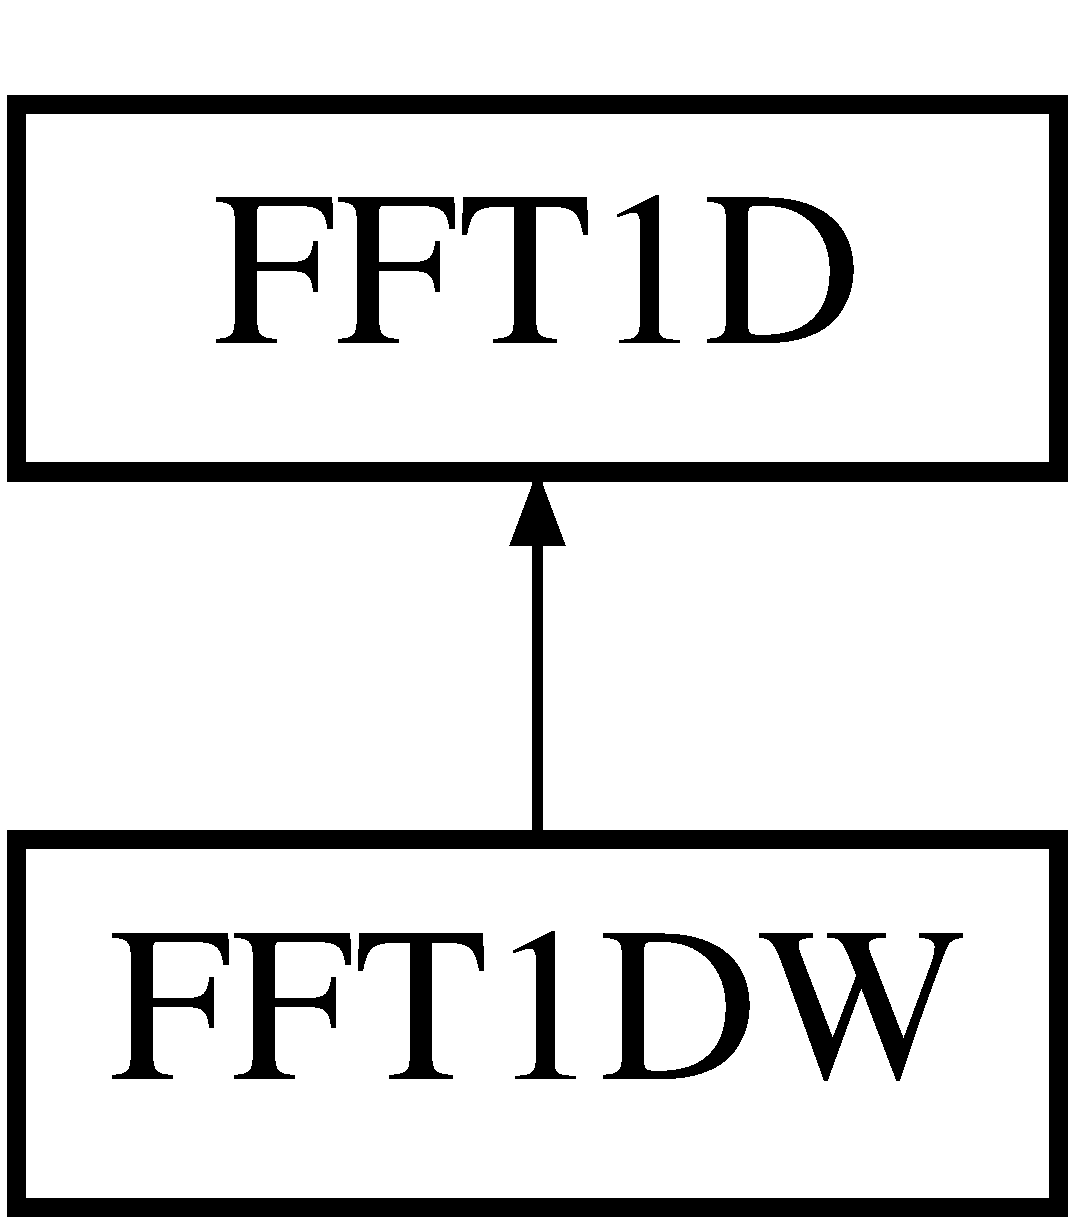
\includegraphics[height=2.000000cm]{class_f_f_t1_d}
\end{center}
\end{figure}
\subsection*{Public Member Functions}
\begin{DoxyCompactItemize}
\item 
\mbox{\Hypertarget{class_f_f_t1_d_a43ff9aee84ed44bb71b8334e41267da8}\label{class_f_f_t1_d_a43ff9aee84ed44bb71b8334e41267da8}} 
{\bfseries F\+F\+T1D} (unsigned int a\+\_\+M)
\item 
\mbox{\Hypertarget{class_f_f_t1_d_a66ca6abdacadd9d77c9d1f39ab508202}\label{class_f_f_t1_d_a66ca6abdacadd9d77c9d1f39ab508202}} 
virtual void {\bfseries forward\+F\+F\+T\+CC} (vector$<$ complex$<$ double $>$ $>$ \&a\+\_\+f\+Hat, const vector$<$ complex$<$ double $>$ $>$ \&f) const =0
\item 
\mbox{\Hypertarget{class_f_f_t1_d_aa8611e6f021a752e60675b33741214c7}\label{class_f_f_t1_d_aa8611e6f021a752e60675b33741214c7}} 
virtual void {\bfseries inverse\+F\+F\+T\+CC} (vector$<$ complex$<$ double $>$ $>$ \&a\+\_\+f, const vector$<$ complex$<$ double $>$ $>$ \&a\+\_\+f\+Hat) const =0
\item 
\mbox{\Hypertarget{class_f_f_t1_d_a808e5d0c9b29c846e1ebff94b8474897}\label{class_f_f_t1_d_a808e5d0c9b29c846e1ebff94b8474897}} 
const unsigned int \& {\bfseries getN} ()
\item 
\mbox{\Hypertarget{class_f_f_t1_d_a4b9470b228d9284224f653f6b0700371}\label{class_f_f_t1_d_a4b9470b228d9284224f653f6b0700371}} 
const unsigned int \& {\bfseries getM} ()
\end{DoxyCompactItemize}
\subsection*{Protected Attributes}
\begin{DoxyCompactItemize}
\item 
\mbox{\Hypertarget{class_f_f_t1_d_a7cc11c775917dc9ab05b87712720a208}\label{class_f_f_t1_d_a7cc11c775917dc9ab05b87712720a208}} 
unsigned int {\bfseries m\+\_\+M}
\item 
\mbox{\Hypertarget{class_f_f_t1_d_ac9b2fd31fea75c4101f658f104ebd182}\label{class_f_f_t1_d_ac9b2fd31fea75c4101f658f104ebd182}} 
unsigned int {\bfseries m\+\_\+N}
\end{DoxyCompactItemize}


The documentation for this class was generated from the following file\+:\begin{DoxyCompactItemize}
\item 
src/fft\+Tools/F\+F\+T1\+D.\+H\end{DoxyCompactItemize}

\hypertarget{class_f_f_t1_d_w}{}\section{F\+F\+T1\+DW Class Reference}
\label{class_f_f_t1_d_w}\index{F\+F\+T1\+DW@{F\+F\+T1\+DW}}
Inheritance diagram for F\+F\+T1\+DW\+:\begin{figure}[H]
\begin{center}
\leavevmode
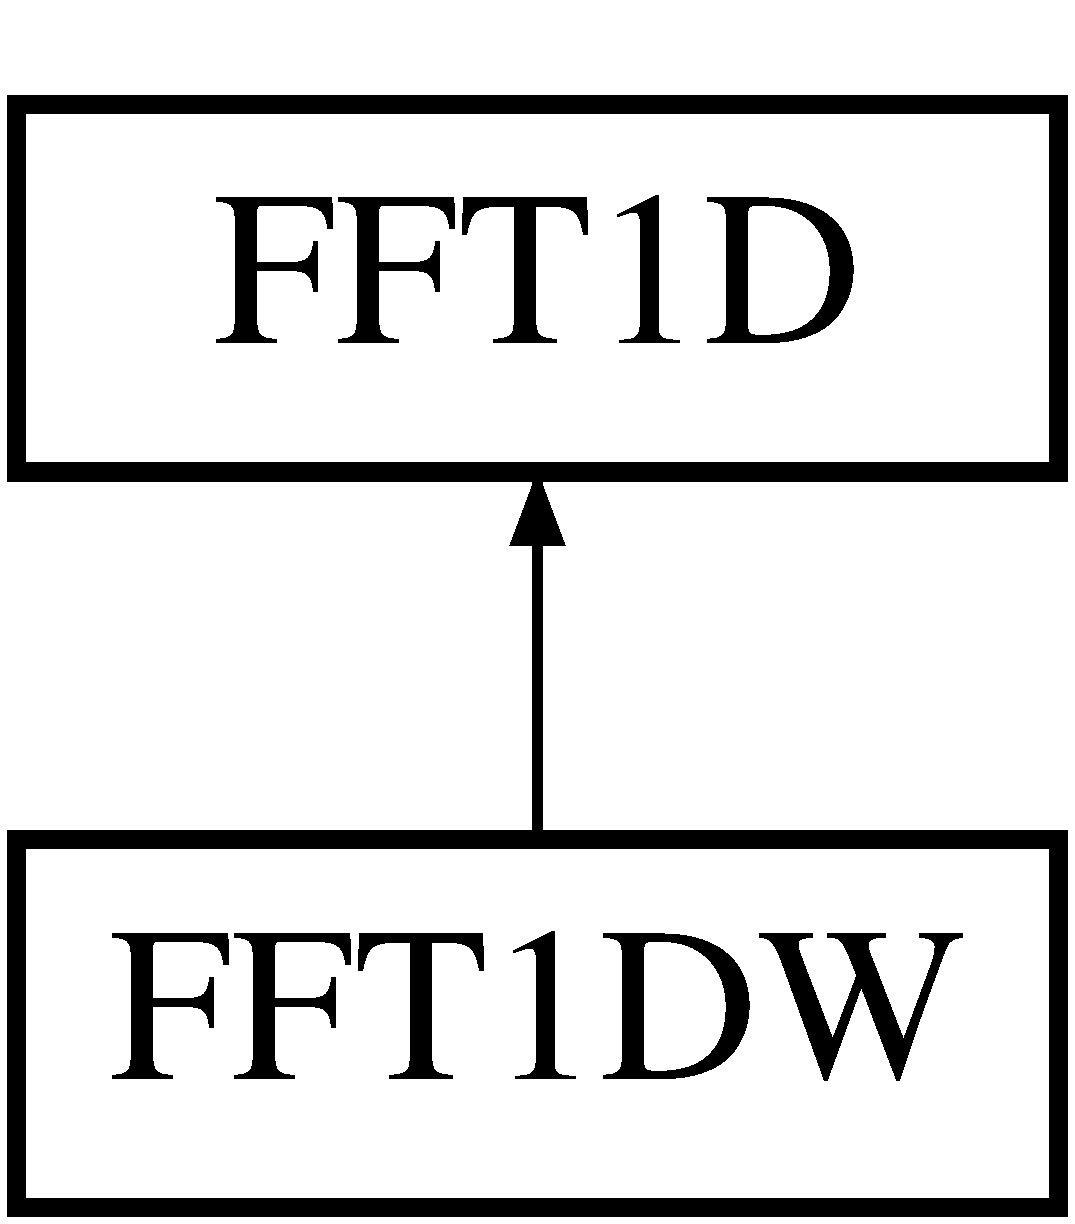
\includegraphics[height=2.000000cm]{class_f_f_t1_d_w}
\end{center}
\end{figure}
\subsection*{Public Member Functions}
\begin{DoxyCompactItemize}
\item 
\mbox{\Hypertarget{class_f_f_t1_d_w_a8ee1895cec2e681fd0f2927e98b7e6be}\label{class_f_f_t1_d_w_a8ee1895cec2e681fd0f2927e98b7e6be}} 
{\bfseries F\+F\+T1\+DW} (unsigned int a\+\_\+M)
\item 
\mbox{\Hypertarget{class_f_f_t1_d_w_accb0b00b28181e1e723a5611331003fe}\label{class_f_f_t1_d_w_accb0b00b28181e1e723a5611331003fe}} 
virtual void {\bfseries forward\+F\+F\+T\+CC} (vector$<$ complex$<$ double $>$ $>$ \&a\+\_\+f\+Hat, const vector$<$ complex$<$ double $>$ $>$ \&f) const
\item 
\mbox{\Hypertarget{class_f_f_t1_d_w_ab3e7120a9966709cbf6095af90c0811f}\label{class_f_f_t1_d_w_ab3e7120a9966709cbf6095af90c0811f}} 
virtual void {\bfseries inverse\+F\+F\+T\+CC} (vector$<$ complex$<$ double $>$ $>$ \&a\+\_\+f, const vector$<$ complex$<$ double $>$ $>$ \&a\+\_\+f\+Hat) const
\end{DoxyCompactItemize}
\subsection*{Protected Attributes}
\begin{DoxyCompactItemize}
\item 
\mbox{\Hypertarget{class_f_f_t1_d_w_a8cbc1a46dca9b0031244a9004f2207a5}\label{class_f_f_t1_d_w_a8cbc1a46dca9b0031244a9004f2207a5}} 
vector$<$ complex$<$ double $>$ $>$ {\bfseries m\+\_\+in}
\item 
\mbox{\Hypertarget{class_f_f_t1_d_w_adf99327f7fb95163620c4f629baf276c}\label{class_f_f_t1_d_w_adf99327f7fb95163620c4f629baf276c}} 
vector$<$ complex$<$ double $>$ $>$ {\bfseries m\+\_\+out}
\item 
\mbox{\Hypertarget{class_f_f_t1_d_w_a2299f3623ee6fe0c5a1f5e354bd9027f}\label{class_f_f_t1_d_w_a2299f3623ee6fe0c5a1f5e354bd9027f}} 
fftw\+\_\+plan {\bfseries m\+\_\+forward}
\item 
\mbox{\Hypertarget{class_f_f_t1_d_w_a471a064f64ecc9dc4d6fba8f61e747c2}\label{class_f_f_t1_d_w_a471a064f64ecc9dc4d6fba8f61e747c2}} 
fftw\+\_\+plan {\bfseries m\+\_\+inverse}
\end{DoxyCompactItemize}


The documentation for this class was generated from the following files\+:\begin{DoxyCompactItemize}
\item 
src/fft\+Tools/F\+F\+T1\+D\+W.\+H\item 
src/fft\+Tools/F\+F\+T1\+D\+W.\+cpp\end{DoxyCompactItemize}

\hypertarget{class_f_f_t_m_d}{}\section{F\+F\+T\+MD Class Reference}
\label{class_f_f_t_m_d}\index{F\+F\+T\+MD@{F\+F\+T\+MD}}
\subsection*{Public Member Functions}
\begin{DoxyCompactItemize}
\item 
\mbox{\Hypertarget{class_f_f_t_m_d_ac1540fd0cca52cec510f8e5cfc4cb222}\label{class_f_f_t_m_d_ac1540fd0cca52cec510f8e5cfc4cb222}} 
{\bfseries F\+F\+T\+MD} (shared\+\_\+ptr$<$ \hyperlink{class_f_f_t1_d}{F\+F\+T1D} $>$ a\+\_\+fft1d\+Ptr)
\item 
\mbox{\Hypertarget{class_f_f_t_m_d_a96afb71bd36d3e970edf77a679a9a3d0}\label{class_f_f_t_m_d_a96afb71bd36d3e970edf77a679a9a3d0}} 
void {\bfseries define} (shared\+\_\+ptr$<$ \hyperlink{class_f_f_t1_d}{F\+F\+T1D} $>$ a\+\_\+fft1d\+Ptr)
\item 
\mbox{\Hypertarget{class_f_f_t_m_d_ac77ccb3251ca36753d8486482e463571}\label{class_f_f_t_m_d_ac77ccb3251ca36753d8486482e463571}} 
void {\bfseries forward\+CC} (\hyperlink{class_rect_m_d_array}{Rect\+M\+D\+Array}$<$ complex$<$ double $>$ $>$ \&a\+\_\+f) const
\item 
\mbox{\Hypertarget{class_f_f_t_m_d_a3a8212aa243e238fe9b6ebc0d75c3b81}\label{class_f_f_t_m_d_a3a8212aa243e238fe9b6ebc0d75c3b81}} 
void {\bfseries inverse\+CC} (\hyperlink{class_rect_m_d_array}{Rect\+M\+D\+Array}$<$ complex$<$ double $>$ $>$ \&a\+\_\+f\+Hat) const
\item 
\mbox{\Hypertarget{class_f_f_t_m_d_af3a20a457873df74597751c41f80d624}\label{class_f_f_t_m_d_af3a20a457873df74597751c41f80d624}} 
void {\bfseries forward\+C\+Ccen} (\hyperlink{class_rect_m_d_array}{Rect\+M\+D\+Array}$<$ complex$<$ double $>$ $>$ \&a\+\_\+f) const
\item 
\mbox{\Hypertarget{class_f_f_t_m_d_a06580a8025af117f54531d83f5e947a5}\label{class_f_f_t_m_d_a06580a8025af117f54531d83f5e947a5}} 
void {\bfseries inverse\+C\+Ccen} (\hyperlink{class_rect_m_d_array}{Rect\+M\+D\+Array}$<$ complex$<$ double $>$ $>$ \&a\+\_\+f\+Hat) const
\item 
\mbox{\Hypertarget{class_f_f_t_m_d_a2f578a9fbeb3d759303a5e4f54530f0b}\label{class_f_f_t_m_d_a2f578a9fbeb3d759303a5e4f54530f0b}} 
const int \& {\bfseries getN} () const
\item 
\mbox{\Hypertarget{class_f_f_t_m_d_a78a693aac85a0ceb5d9961c26b3ed704}\label{class_f_f_t_m_d_a78a693aac85a0ceb5d9961c26b3ed704}} 
const int \& {\bfseries getM} () const
\end{DoxyCompactItemize}


The documentation for this class was generated from the following files\+:\begin{DoxyCompactItemize}
\item 
src/fft\+Tools/F\+F\+T\+M\+D.\+H\item 
src/fft\+Tools/F\+F\+T\+M\+D.\+cpp\end{DoxyCompactItemize}

\hypertarget{class_hockney}{}\section{Hockney Class Reference}
\label{class_hockney}\index{Hockney@{Hockney}}
\subsection*{Public Member Functions}
\begin{DoxyCompactItemize}
\item 
\mbox{\Hypertarget{class_hockney_a6f65a0f28be1522faa7dbe8edbefb1ab}\label{class_hockney_a6f65a0f28be1522faa7dbe8edbefb1ab}} 
{\bfseries Hockney} (shared\+\_\+ptr$<$ \hyperlink{class_conv_kernel}{Conv\+Kernel} $>$ \&a\+\_\+ker\+Ptr, const double \&a\+\_\+h, int a\+\_\+M)
\item 
\mbox{\Hypertarget{class_hockney_a845942d3dc47756860aff77afb89499f}\label{class_hockney_a845942d3dc47756860aff77afb89499f}} 
void {\bfseries define} (shared\+\_\+ptr$<$ \hyperlink{class_conv_kernel}{Conv\+Kernel} $>$ \&a\+\_\+ker\+Ptr, const double \&a\+\_\+h, int a\+\_\+M)
\item 
\mbox{\Hypertarget{class_hockney_a42de9a1d8871a7d082985633718c9683}\label{class_hockney_a42de9a1d8871a7d082985633718c9683}} 
void {\bfseries convolve} (\hyperlink{class_rect_m_d_array}{Rect\+M\+D\+Array}$<$ double $>$ \&a\+\_\+rhs)
\end{DoxyCompactItemize}
\subsection*{Protected Attributes}
\begin{DoxyCompactItemize}
\item 
\mbox{\Hypertarget{class_hockney_a117b101e4d0e7c21be97b54567ce025d}\label{class_hockney_a117b101e4d0e7c21be97b54567ce025d}} 
double {\bfseries m\+\_\+h}
\item 
\mbox{\Hypertarget{class_hockney_a285ed890fe7fa49e984359cb7d608633}\label{class_hockney_a285ed890fe7fa49e984359cb7d608633}} 
int {\bfseries m\+\_\+M}
\item 
\mbox{\Hypertarget{class_hockney_a457e33c833c6624297875c1ff1991f31}\label{class_hockney_a457e33c833c6624297875c1ff1991f31}} 
int {\bfseries m\+\_\+N}
\item 
\mbox{\Hypertarget{class_hockney_a94cc01535b5865bdac9a1355aba65bb4}\label{class_hockney_a94cc01535b5865bdac9a1355aba65bb4}} 
\hyperlink{class_f_f_t_m_d}{F\+F\+T\+MD} {\bfseries m\+\_\+fftmd}
\item 
\mbox{\Hypertarget{class_hockney_abfd66c7ddccd95686f9d7394d37df3b7}\label{class_hockney_abfd66c7ddccd95686f9d7394d37df3b7}} 
shared\+\_\+ptr$<$ \hyperlink{class_conv_kernel}{Conv\+Kernel} $>$ {\bfseries m\+\_\+ker\+Ptr}
\item 
\mbox{\Hypertarget{class_hockney_a90187a035100a4ad48d43e53dc6e169f}\label{class_hockney_a90187a035100a4ad48d43e53dc6e169f}} 
bool {\bfseries m\+\_\+is\+Defined}
\end{DoxyCompactItemize}


The documentation for this class was generated from the following files\+:\begin{DoxyCompactItemize}
\item 
src/\+Hockney/Hockney.\+H\item 
src/\+Hockney/Hockney.\+cpp\end{DoxyCompactItemize}

\hypertarget{class_particle}{}\section{Particle Class Reference}
\label{class_particle}\index{Particle@{Particle}}


Represents a single particle in a \hyperlink{class_particle_set}{Particle\+Set}.  




{\ttfamily \#include $<$Particle.\+H$>$}

\subsection*{Public Member Functions}
\begin{DoxyCompactItemize}
\item 
\mbox{\Hypertarget{class_particle_a6f0bab4db5e06324b46ea10927059306}\label{class_particle_a6f0bab4db5e06324b46ea10927059306}} 
void \hyperlink{class_particle_a6f0bab4db5e06324b46ea10927059306}{increment} (const \hyperlink{class_d_x}{DX} \&a\+\_\+shift)
\begin{DoxyCompactList}\small\item\em used to implement \hyperlink{class_particle_set_aa27ac22706a979dd57b6523254b27d83}{Particle\+Set\+::increment}. \end{DoxyCompactList}\end{DoxyCompactItemize}
\subsection*{Public Attributes}
\begin{DoxyCompactItemize}
\item 
\mbox{\Hypertarget{class_particle_a70fbd1aa4ee14710ab1e2f2cf5bdc211}\label{class_particle_a70fbd1aa4ee14710ab1e2f2cf5bdc211}} 
array$<$ double, D\+IM $>$ \hyperlink{class_particle_a70fbd1aa4ee14710ab1e2f2cf5bdc211}{m\+\_\+x}
\begin{DoxyCompactList}\small\item\em m\+\_\+x stores the spatial location of the particle, and strength the vorticity. \end{DoxyCompactList}\item 
\mbox{\Hypertarget{class_particle_a8de58af6e42f14ba1ffefc2007498bbf}\label{class_particle_a8de58af6e42f14ba1ffefc2007498bbf}} 
double {\bfseries strength}
\end{DoxyCompactItemize}


\subsection{Detailed Description}
Represents a single particle in a \hyperlink{class_particle_set}{Particle\+Set}. 

The documentation for this class was generated from the following file\+:\begin{DoxyCompactItemize}
\item 
src/\+Particles/Particle.\+H\end{DoxyCompactItemize}

\hypertarget{class_particle_set}{}\section{Particle\+Set Class Reference}
\label{class_particle_set}\index{Particle\+Set@{Particle\+Set}}


Represents a collection of particles, conforming to the X class in \hyperlink{class_r_k4}{R\+K4}. Also contains the persistent data required to compute the right-\/hand side in Particles\+Velocities.  




{\ttfamily \#include $<$Particle\+Set.\+H$>$}

\subsection*{Public Member Functions}
\begin{DoxyCompactItemize}
\item 
\hyperlink{class_particle_set_a3963fc6e57575ff7702b96fa2b5f1ccb}{Particle\+Set} (shared\+\_\+ptr$<$ \hyperlink{class_conv_kernel}{Conv\+Kernel} $>$ \&a\+\_\+kerptr, \hyperlink{class_d_box}{D\+Box} \&a\+\_\+box, double \&a\+\_\+dx, array$<$ double, D\+IM $>$ \&a\+\_\+low\+Corner, int a\+\_\+M)
\begin{DoxyCompactList}\small\item\em constructor. Called by main. \end{DoxyCompactList}\item 
\mbox{\Hypertarget{class_particle_set_aa27ac22706a979dd57b6523254b27d83}\label{class_particle_set_aa27ac22706a979dd57b6523254b27d83}} 
void \hyperlink{class_particle_set_aa27ac22706a979dd57b6523254b27d83}{increment} (const \hyperlink{class_particle_shift}{Particle\+Shift} \&a\+\_\+shift)
\begin{DoxyCompactList}\small\item\em inplements increment function required for RK\$. \end{DoxyCompactList}\end{DoxyCompactItemize}
\subsection*{Public Attributes}
\begin{DoxyCompactItemize}
\item 
\mbox{\Hypertarget{class_particle_set_a6bb49eed6fe60ce44d9639cccc49d3fc}\label{class_particle_set_a6bb49eed6fe60ce44d9639cccc49d3fc}} 
vector$<$ \hyperlink{class_particle}{Particle} $>$ \hyperlink{class_particle_set_a6bb49eed6fe60ce44d9639cccc49d3fc}{m\+\_\+particles}
\begin{DoxyCompactList}\small\item\em Main container for particle data. \end{DoxyCompactList}\item 
\mbox{\Hypertarget{class_particle_set_ab175df8fab554a1c069dc75330bd7ffb}\label{class_particle_set_ab175df8fab554a1c069dc75330bd7ffb}} 
double \hyperlink{class_particle_set_ab175df8fab554a1c069dc75330bd7ffb}{m\+\_\+dx}
\begin{DoxyCompactList}\small\item\em Mesh spacing. \end{DoxyCompactList}\item 
\mbox{\Hypertarget{class_particle_set_ae965763dcc0f6bca9a0d5ed6864ba581}\label{class_particle_set_ae965763dcc0f6bca9a0d5ed6864ba581}} 
\hyperlink{class_d_box}{D\+Box} \hyperlink{class_particle_set_ae965763dcc0f6bca9a0d5ed6864ba581}{m\+\_\+box}
\begin{DoxyCompactList}\small\item\em P\+IC grid. \end{DoxyCompactList}\item 
\mbox{\Hypertarget{class_particle_set_ae99b4064e3ee714f1d1e217c4fb519c6}\label{class_particle_set_ae99b4064e3ee714f1d1e217c4fb519c6}} 
array$<$ double, D\+IM $>$ \hyperlink{class_particle_set_ae99b4064e3ee714f1d1e217c4fb519c6}{m\+\_\+low\+Corner}
\begin{DoxyCompactList}\small\item\em Location in physical space of m\+\_\+box.\+m\+\_\+low\+Corner;. \end{DoxyCompactList}\item 
\mbox{\Hypertarget{class_particle_set_a681f750458d3c20a5e8685f1521cdbf0}\label{class_particle_set_a681f750458d3c20a5e8685f1521cdbf0}} 
\hyperlink{class_hockney}{Hockney} \hyperlink{class_particle_set_a681f750458d3c20a5e8685f1521cdbf0}{m\+\_\+hockney}
\begin{DoxyCompactList}\small\item\em \hyperlink{class_hockney}{Hockney} class that performs discrete convolution. \end{DoxyCompactList}\end{DoxyCompactItemize}


\subsection{Detailed Description}
Represents a collection of particles, conforming to the X class in \hyperlink{class_r_k4}{R\+K4}. Also contains the persistent data required to compute the right-\/hand side in Particles\+Velocities. 

\subsection{Constructor \& Destructor Documentation}
\mbox{\Hypertarget{class_particle_set_a3963fc6e57575ff7702b96fa2b5f1ccb}\label{class_particle_set_a3963fc6e57575ff7702b96fa2b5f1ccb}} 
\index{Particle\+Set@{Particle\+Set}!Particle\+Set@{Particle\+Set}}
\index{Particle\+Set@{Particle\+Set}!Particle\+Set@{Particle\+Set}}
\subsubsection{\texorpdfstring{Particle\+Set()}{ParticleSet()}}
{\footnotesize\ttfamily Particle\+Set\+::\+Particle\+Set (\begin{DoxyParamCaption}\item[{shared\+\_\+ptr$<$ \hyperlink{class_conv_kernel}{Conv\+Kernel} $>$ \&}]{a\+\_\+kerptr,  }\item[{\hyperlink{class_d_box}{D\+Box} \&}]{a\+\_\+box,  }\item[{double \&}]{a\+\_\+dx,  }\item[{array$<$ double, D\+IM $>$ \&}]{a\+\_\+low\+Corner,  }\item[{int}]{a\+\_\+M }\end{DoxyParamCaption})}



constructor. Called by main. 

a\+\_\+kerptr\+: required to construct \hyperlink{class_hockney}{Hockney}. a\+\_\+box\+: \hyperlink{class_d_box}{D\+Box} over which convolution is performed. a\+\_\+dx\+: mesh spacing of P\+IC grid. a\+\_\+low\+Corner\+: D\+I\+M-\/tuple giving the location in physical space of the low\+Corner of the P\+IC grid. a\+\_\+M\+: N = 2$^\wedge$a\+\_\+M is the number of grid points in the P\+IC grid. 

The documentation for this class was generated from the following file\+:\begin{DoxyCompactItemize}
\item 
src/\+Particles/Particle\+Set.\+H\end{DoxyCompactItemize}

\hypertarget{class_particle_shift}{}\section{Particle\+Shift Class Reference}
\label{class_particle_shift}\index{Particle\+Shift@{Particle\+Shift}}


Represents an increment in a \hyperlink{class_particle_set}{Particle\+Set} conforming to the dX class in \hyperlink{class_r_k4}{R\+K4}.  




{\ttfamily \#include $<$Particle\+Set.\+H$>$}

\subsection*{Public Member Functions}
\begin{DoxyCompactItemize}
\item 
\mbox{\Hypertarget{class_particle_shift_aa298bec75ebcd7a6d39285dcc734927c}\label{class_particle_shift_aa298bec75ebcd7a6d39285dcc734927c}} 
void \hyperlink{class_particle_shift_aa298bec75ebcd7a6d39285dcc734927c}{init} (const \hyperlink{class_particle_set}{Particle\+Set} \&a\+\_\+particles)
\begin{DoxyCompactList}\small\item\em Sets length of m\+\_\+particles, initializes to zero via default constructor of \hyperlink{class_d_x}{DX}. \end{DoxyCompactList}\item 
\mbox{\Hypertarget{class_particle_shift_a6f49ef57c1b4a140abacaca103572be3}\label{class_particle_shift_a6f49ef57c1b4a140abacaca103572be3}} 
void \hyperlink{class_particle_shift_a6f49ef57c1b4a140abacaca103572be3}{increment} (double a\+\_\+scale, const \hyperlink{class_particle_shift}{Particle\+Shift} \&a\+\_\+rhs)
\begin{DoxyCompactList}\small\item\em m\+\_\+particles\mbox{[}k\mbox{]} += a\+\_\+rhs.\+m\+\_\+particles\mbox{[}k\mbox{]}$\ast$a\+\_\+scale. \end{DoxyCompactList}\item 
\mbox{\Hypertarget{class_particle_shift_a8ffb0054d1822d05793b68c5e874f3a0}\label{class_particle_shift_a8ffb0054d1822d05793b68c5e874f3a0}} 
void \hyperlink{class_particle_shift_a8ffb0054d1822d05793b68c5e874f3a0}{operator$\ast$=} (double a\+\_\+scale)
\begin{DoxyCompactList}\small\item\em m\+\_\+particles\mbox{[}k\mbox{]} $\ast$= a\+\_\+scale \end{DoxyCompactList}\item 
\mbox{\Hypertarget{class_particle_shift_a4931a6bc6358b26d5e5e48029540c6c5}\label{class_particle_shift_a4931a6bc6358b26d5e5e48029540c6c5}} 
void \hyperlink{class_particle_shift_a4931a6bc6358b26d5e5e48029540c6c5}{set\+To\+Zero} ()
\begin{DoxyCompactList}\small\item\em reinitializes the values m\+\_\+particles\mbox{[}k\mbox{]} to zero. Not used in \hyperlink{class_r_k4}{R\+K4}. \end{DoxyCompactList}\end{DoxyCompactItemize}
\subsection*{Public Attributes}
\begin{DoxyCompactItemize}
\item 
\mbox{\Hypertarget{class_particle_shift_ace15f1432744690f40f43fe2a5016e64}\label{class_particle_shift_ace15f1432744690f40f43fe2a5016e64}} 
vector$<$ \hyperlink{class_d_x}{DX} $>$ \hyperlink{class_particle_shift_ace15f1432744690f40f43fe2a5016e64}{m\+\_\+particles}
\begin{DoxyCompactList}\small\item\em vector of increments of particles. \end{DoxyCompactList}\end{DoxyCompactItemize}


\subsection{Detailed Description}
Represents an increment in a \hyperlink{class_particle_set}{Particle\+Set} conforming to the dX class in \hyperlink{class_r_k4}{R\+K4}. 

The documentation for this class was generated from the following file\+:\begin{DoxyCompactItemize}
\item 
src/\+Particles/Particle\+Set.\+H\end{DoxyCompactItemize}

\hypertarget{class_particle_velocities}{}\section{Particle\+Velocities Class Reference}
\label{class_particle_velocities}\index{Particle\+Velocities@{Particle\+Velocities}}


Class for computing the R\+HS in \hyperlink{class_r_k4}{R\+K4}, corresponding to the template parameter F.  




{\ttfamily \#include $<$Particle\+Velocities.\+H$>$}

\subsection*{Public Member Functions}
\begin{DoxyCompactItemize}
\item 
\hyperlink{class_particle_velocities_a10b68a5a7868192c508bc2b4a492aa51}{Particle\+Velocities} ()
\begin{DoxyCompactList}\small\item\em Member function that computes increment to solution.\+Conforms to the m\+\_\+f(...) interface in \hyperlink{class_r_k4}{R\+K4}. \end{DoxyCompactList}\item 
\mbox{\Hypertarget{class_particle_velocities_a72b8fd71b794e841c5f67dc2b728dec1}\label{class_particle_velocities_a72b8fd71b794e841c5f67dc2b728dec1}} 
void {\bfseries operator()} (\hyperlink{class_particle_shift}{Particle\+Shift} \&a\+\_\+k, const double \&a\+\_\+time, const double \&dt, \hyperlink{class_particle_set}{Particle\+Set} \&a\+\_\+state)
\end{DoxyCompactItemize}


\subsection{Detailed Description}
Class for computing the R\+HS in \hyperlink{class_r_k4}{R\+K4}, corresponding to the template parameter F. 

\subsection{Constructor \& Destructor Documentation}
\mbox{\Hypertarget{class_particle_velocities_a10b68a5a7868192c508bc2b4a492aa51}\label{class_particle_velocities_a10b68a5a7868192c508bc2b4a492aa51}} 
\index{Particle\+Velocities@{Particle\+Velocities}!Particle\+Velocities@{Particle\+Velocities}}
\index{Particle\+Velocities@{Particle\+Velocities}!Particle\+Velocities@{Particle\+Velocities}}
\subsubsection{\texorpdfstring{Particle\+Velocities()}{ParticleVelocities()}}
{\footnotesize\ttfamily Particle\+Velocities\+::\+Particle\+Velocities (\begin{DoxyParamCaption}{ }\end{DoxyParamCaption})}



Member function that computes increment to solution.\+Conforms to the m\+\_\+f(...) interface in \hyperlink{class_r_k4}{R\+K4}. 

Implements an operator that evaluates a\+\_\+dt$\ast$F(t,a\+\_\+\+X+a\+\_\+k), given the inputs (a\+\_\+k, a\+\_\+time, a\+\_\+dt, a\+\_\+X ). It first computes a temporary a\+\_\+X + a\+\_\+k, then evaluates the right-\/hand side, scales the result by a\+\_\+dt and stores it in a\+\_\+k. 

The documentation for this class was generated from the following file\+:\begin{DoxyCompactItemize}
\item 
src/\+Particles/Particle\+Velocities.\+H\end{DoxyCompactItemize}

\hypertarget{class_point}{}\section{Point Class Reference}
\label{class_point}\index{Point@{Point}}


A point in space.  




{\ttfamily \#include $<$Point.\+H$>$}

\subsection*{Public Member Functions}
\begin{DoxyCompactItemize}
\item 
\mbox{\Hypertarget{class_point_ad92f2337b839a94ce97dcdb439b4325a}\label{class_point_ad92f2337b839a94ce97dcdb439b4325a}} 
\hyperlink{class_point_ad92f2337b839a94ce97dcdb439b4325a}{Point} ()
\begin{DoxyCompactList}\small\item\em Default Constructor. \end{DoxyCompactList}\item 
\mbox{\Hypertarget{class_point_ad2979175ac77062182ecfae283c8b97f}\label{class_point_ad2979175ac77062182ecfae283c8b97f}} 
\hyperlink{class_point_ad2979175ac77062182ecfae283c8b97f}{Point} (const int a\+\_\+tuple\mbox{[}D\+IM\mbox{]})
\begin{DoxyCompactList}\small\item\em Construct a \hyperlink{class_point}{Point} using an int array. \end{DoxyCompactList}\item 
\mbox{\Hypertarget{class_point_abaef269e1437aab4ed03ba64b4fafaa2}\label{class_point_abaef269e1437aab4ed03ba64b4fafaa2}} 
\hyperlink{class_point_abaef269e1437aab4ed03ba64b4fafaa2}{Point} (const array$<$ int, D\+IM $>$ a\+\_\+tuple)
\begin{DoxyCompactList}\small\item\em Construct a \hyperlink{class_point}{Point} using a std\+::array of ints. \end{DoxyCompactList}\item 
\mbox{\Hypertarget{class_point_ad3049b9597a2dc93be3fc304bbf3cdbb}\label{class_point_ad3049b9597a2dc93be3fc304bbf3cdbb}} 
\hyperlink{class_point_ad3049b9597a2dc93be3fc304bbf3cdbb}{Point} (const \hyperlink{class_point}{Point} \&a\+\_\+pt)
\begin{DoxyCompactList}\small\item\em Copy Constructor. \end{DoxyCompactList}\item 
bool \hyperlink{class_point_ab93641cb4a786c87778c63ad23e9ec0b}{operator$<$} (const \hyperlink{class_point}{Point} \&a\+\_\+rhs) const
\begin{DoxyCompactList}\small\item\em Definition of \char`\"{}$<$\char`\"{} operator on Points. Returns true if this$\ast$ is \char`\"{}less than\char`\"{} $\ast$a\+\_\+rhs. \end{DoxyCompactList}\item 
\mbox{\Hypertarget{class_point_a33ef2fd0c9e91605f6cd986e99e9fd06}\label{class_point_a33ef2fd0c9e91605f6cd986e99e9fd06}} 
\hyperlink{class_point}{Point} \hyperlink{class_point_a33ef2fd0c9e91605f6cd986e99e9fd06}{operator+} (const \hyperlink{class_point}{Point} \&a\+\_\+rhs\+Point) const
\begin{DoxyCompactList}\small\item\em Componentwise addition of two Points. \end{DoxyCompactList}\item 
\mbox{\Hypertarget{class_point_a2d918abfc8d84e03b890878778180fd3}\label{class_point_a2d918abfc8d84e03b890878778180fd3}} 
\hyperlink{class_point}{Point} \hyperlink{class_point_a2d918abfc8d84e03b890878778180fd3}{operator-\/} (const \hyperlink{class_point}{Point} \&a\+\_\+rhs\+Point) const
\begin{DoxyCompactList}\small\item\em Componentwise subtraction of two Points. \end{DoxyCompactList}\item 
\hyperlink{class_point}{Point} \hyperlink{class_point_a4f8c24c02a61c5727fa4e049638feba7}{operator/} (int a\+\_\+nref) const
\begin{DoxyCompactList}\small\item\em Componentwise division of a \hyperlink{class_point}{Point} by an Integer. \end{DoxyCompactList}\item 
\hyperlink{class_point}{Point} \hyperlink{class_point_a15d362c09b31d632a0f3cd5e7a96eef7}{operator/} (const \hyperlink{class_point}{Point} \&a\+\_\+pt) const
\begin{DoxyCompactList}\small\item\em Componentwise division of a \hyperlink{class_point}{Point} by another \hyperlink{class_point}{Point}. \end{DoxyCompactList}\item 
\mbox{\Hypertarget{class_point_a0e08b54dfb11c2c54907eb0b6aa54dae}\label{class_point_a0e08b54dfb11c2c54907eb0b6aa54dae}} 
\hyperlink{class_point}{Point} \hyperlink{class_point_a0e08b54dfb11c2c54907eb0b6aa54dae}{operator$\ast$} (int a\+\_\+nref) const
\begin{DoxyCompactList}\small\item\em Componentwise multiplication of a \hyperlink{class_point}{Point} by an Integer. \end{DoxyCompactList}\item 
\mbox{\Hypertarget{class_point_a2db4fa18cb39589963aacca00636dbe5}\label{class_point_a2db4fa18cb39589963aacca00636dbe5}} 
\hyperlink{class_point}{Point} \hyperlink{class_point_a2db4fa18cb39589963aacca00636dbe5}{operator$\ast$} (const \hyperlink{class_point}{Point} \&a\+\_\+pt) const
\begin{DoxyCompactList}\small\item\em Componentwise multiplication between two Points. \end{DoxyCompactList}\item 
\mbox{\Hypertarget{class_point_ab7db9ac762d6637efcce56afc7750f1f}\label{class_point_ab7db9ac762d6637efcce56afc7750f1f}} 
void \hyperlink{class_point_ab7db9ac762d6637efcce56afc7750f1f}{operator$\ast$=} (const \hyperlink{class_point}{Point} \&a\+\_\+pt)
\begin{DoxyCompactList}\small\item\em Multiplication of two Points in place. \end{DoxyCompactList}\item 
\mbox{\Hypertarget{class_point_a587465b64c61c24c7bcb9abf0dfda114}\label{class_point_a587465b64c61c24c7bcb9abf0dfda114}} 
void \hyperlink{class_point_a587465b64c61c24c7bcb9abf0dfda114}{operator+=} (const \hyperlink{class_point}{Point} \&a\+\_\+pt)
\begin{DoxyCompactList}\small\item\em Addition of two Points in place. \end{DoxyCompactList}\item 
\mbox{\Hypertarget{class_point_a5c41a95bd50b076bdca75d920f73554f}\label{class_point_a5c41a95bd50b076bdca75d920f73554f}} 
void \hyperlink{class_point_a5c41a95bd50b076bdca75d920f73554f}{operator-\/=} (const \hyperlink{class_point}{Point} \&a\+\_\+pt)
\begin{DoxyCompactList}\small\item\em Subtraction of two Points in place. \end{DoxyCompactList}\item 
void \hyperlink{class_point_a61672dab6c26441eac5aca9928cdfc1f}{operator/=} (const \hyperlink{class_point}{Point} \&a\+\_\+pt)
\begin{DoxyCompactList}\small\item\em Division of two Points in place. \end{DoxyCompactList}\item 
\mbox{\Hypertarget{class_point_a79d9895cf934366e864a69a483e5b8ad}\label{class_point_a79d9895cf934366e864a69a483e5b8ad}} 
void \hyperlink{class_point_a79d9895cf934366e864a69a483e5b8ad}{operator$\ast$=} (int a\+\_\+n)
\begin{DoxyCompactList}\small\item\em Multiplication in place by an Integer. \end{DoxyCompactList}\item 
\mbox{\Hypertarget{class_point_ae6e49461a0bc525c0f55bd5ce42db45b}\label{class_point_ae6e49461a0bc525c0f55bd5ce42db45b}} 
void \hyperlink{class_point_ae6e49461a0bc525c0f55bd5ce42db45b}{operator+=} (int a\+\_\+n)
\begin{DoxyCompactList}\small\item\em Addition in place by an Integer. \end{DoxyCompactList}\item 
\mbox{\Hypertarget{class_point_a880f2ce648e6011177058678f6b2021b}\label{class_point_a880f2ce648e6011177058678f6b2021b}} 
void \hyperlink{class_point_a880f2ce648e6011177058678f6b2021b}{operator-\/=} (int a\+\_\+n)
\begin{DoxyCompactList}\small\item\em Subtraction in place by an Integer. \end{DoxyCompactList}\item 
void \hyperlink{class_point_a62ab14874fced136ff69ed4cf6d34c90}{operator/=} (int a\+\_\+n)
\begin{DoxyCompactList}\small\item\em Division in place by an Integer. \end{DoxyCompactList}\item 
bool \hyperlink{class_point_a8cf841adb026628dda2df391952ece75}{operator==} (const \hyperlink{class_point}{Point} \&a\+\_\+pt) const
\begin{DoxyCompactList}\small\item\em Equality between two Points. \end{DoxyCompactList}\item 
bool \hyperlink{class_point_abc6eed13223637f36a7d00adadb20931}{operator!=} (const \hyperlink{class_point}{Point} \&a\+\_\+pt) const
\begin{DoxyCompactList}\small\item\em Inequality between two Points. \end{DoxyCompactList}\item 
const int \& \hyperlink{class_point_a267f1f8120637239e6486bdae0ad48e0}{operator\mbox{[}$\,$\mbox{]}} (unsigned char a\+\_\+index) const
\begin{DoxyCompactList}\small\item\em Get component of $\ast$this corresponding to a\+\_\+index. \end{DoxyCompactList}\item 
\mbox{\Hypertarget{class_point_aa92158a649554fe87ccf3c2cf4065737}\label{class_point_aa92158a649554fe87ccf3c2cf4065737}} 
int \& \hyperlink{class_point_aa92158a649554fe87ccf3c2cf4065737}{operator\mbox{[}$\,$\mbox{]}} (unsigned char a\+\_\+index)
\begin{DoxyCompactList}\small\item\em Get component of $\ast$this corresponding to a\+\_\+index. \end{DoxyCompactList}\item 
void \hyperlink{class_point_ae1b141ad286025fc7b4183cc27ef8c0d}{print} () const
\begin{DoxyCompactList}\small\item\em Print out the contents of a \hyperlink{class_point}{Point}. \end{DoxyCompactList}\item 
void \hyperlink{class_point_a8d35b17f0c98a44464926cf605e3d7b6}{print2} () const
\begin{DoxyCompactList}\small\item\em Print out the contents of a \hyperlink{class_point}{Point}. \end{DoxyCompactList}\end{DoxyCompactItemize}


\subsection{Detailed Description}
A point in space. 

An Integer valued point in space of arbitrary dimension. Used to represent Points in a rectangular grid. 

\subsection{Member Function Documentation}
\mbox{\Hypertarget{class_point_abc6eed13223637f36a7d00adadb20931}\label{class_point_abc6eed13223637f36a7d00adadb20931}} 
\index{Point@{Point}!operator"!=@{operator"!=}}
\index{operator"!=@{operator"!=}!Point@{Point}}
\subsubsection{\texorpdfstring{operator"!=()}{operator!=()}}
{\footnotesize\ttfamily bool Point\+::operator!= (\begin{DoxyParamCaption}\item[{const \hyperlink{class_point}{Point} \&}]{a\+\_\+pt }\end{DoxyParamCaption}) const\hspace{0.3cm}{\ttfamily [inline]}}



Inequality between two Points. 

Returns false if $\ast$this == $\ast$a\+\_\+pt. \mbox{\Hypertarget{class_point_a4f8c24c02a61c5727fa4e049638feba7}\label{class_point_a4f8c24c02a61c5727fa4e049638feba7}} 
\index{Point@{Point}!operator/@{operator/}}
\index{operator/@{operator/}!Point@{Point}}
\subsubsection{\texorpdfstring{operator/()}{operator/()}\hspace{0.1cm}{\footnotesize\ttfamily [1/2]}}
{\footnotesize\ttfamily \hyperlink{class_point}{Point} Point\+::operator/ (\begin{DoxyParamCaption}\item[{int}]{a\+\_\+nref }\end{DoxyParamCaption}) const\hspace{0.3cm}{\ttfamily [inline]}}



Componentwise division of a \hyperlink{class_point}{Point} by an Integer. 

Quotients are rounded down. Division of any component by 0 yields an error. \mbox{\Hypertarget{class_point_a15d362c09b31d632a0f3cd5e7a96eef7}\label{class_point_a15d362c09b31d632a0f3cd5e7a96eef7}} 
\index{Point@{Point}!operator/@{operator/}}
\index{operator/@{operator/}!Point@{Point}}
\subsubsection{\texorpdfstring{operator/()}{operator/()}\hspace{0.1cm}{\footnotesize\ttfamily [2/2]}}
{\footnotesize\ttfamily \hyperlink{class_point}{Point} Point\+::operator/ (\begin{DoxyParamCaption}\item[{const \hyperlink{class_point}{Point} \&}]{a\+\_\+pt }\end{DoxyParamCaption}) const\hspace{0.3cm}{\ttfamily [inline]}}



Componentwise division of a \hyperlink{class_point}{Point} by another \hyperlink{class_point}{Point}. 

Quotients are rounded down. Division of any component by 0 yields an error. \mbox{\Hypertarget{class_point_a61672dab6c26441eac5aca9928cdfc1f}\label{class_point_a61672dab6c26441eac5aca9928cdfc1f}} 
\index{Point@{Point}!operator/=@{operator/=}}
\index{operator/=@{operator/=}!Point@{Point}}
\subsubsection{\texorpdfstring{operator/=()}{operator/=()}\hspace{0.1cm}{\footnotesize\ttfamily [1/2]}}
{\footnotesize\ttfamily void Point\+::operator/= (\begin{DoxyParamCaption}\item[{const \hyperlink{class_point}{Point} \&}]{a\+\_\+pt }\end{DoxyParamCaption})\hspace{0.3cm}{\ttfamily [inline]}}



Division of two Points in place. 

Quotients are rounded down. Division of any component by 0 yields an error. \mbox{\Hypertarget{class_point_a62ab14874fced136ff69ed4cf6d34c90}\label{class_point_a62ab14874fced136ff69ed4cf6d34c90}} 
\index{Point@{Point}!operator/=@{operator/=}}
\index{operator/=@{operator/=}!Point@{Point}}
\subsubsection{\texorpdfstring{operator/=()}{operator/=()}\hspace{0.1cm}{\footnotesize\ttfamily [2/2]}}
{\footnotesize\ttfamily void Point\+::operator/= (\begin{DoxyParamCaption}\item[{int}]{a\+\_\+n }\end{DoxyParamCaption})\hspace{0.3cm}{\ttfamily [inline]}}



Division in place by an Integer. 

Quotients are rounded down. Division of any component by 0 yields an error. \mbox{\Hypertarget{class_point_ab93641cb4a786c87778c63ad23e9ec0b}\label{class_point_ab93641cb4a786c87778c63ad23e9ec0b}} 
\index{Point@{Point}!operator$<$@{operator$<$}}
\index{operator$<$@{operator$<$}!Point@{Point}}
\subsubsection{\texorpdfstring{operator$<$()}{operator<()}}
{\footnotesize\ttfamily bool Point\+::operator$<$ (\begin{DoxyParamCaption}\item[{const \hyperlink{class_point}{Point} \&}]{a\+\_\+rhs }\end{DoxyParamCaption}) const\hspace{0.3cm}{\ttfamily [inline]}}



Definition of \char`\"{}$<$\char`\"{} operator on Points. Returns true if this$\ast$ is \char`\"{}less than\char`\"{} $\ast$a\+\_\+rhs. 

This is just an ordering. It is used to add Points to maps etc. Don\textquotesingle{}t use it to actually compare Points. \mbox{\Hypertarget{class_point_a8cf841adb026628dda2df391952ece75}\label{class_point_a8cf841adb026628dda2df391952ece75}} 
\index{Point@{Point}!operator==@{operator==}}
\index{operator==@{operator==}!Point@{Point}}
\subsubsection{\texorpdfstring{operator==()}{operator==()}}
{\footnotesize\ttfamily bool Point\+::operator== (\begin{DoxyParamCaption}\item[{const \hyperlink{class_point}{Point} \&}]{a\+\_\+pt }\end{DoxyParamCaption}) const\hspace{0.3cm}{\ttfamily [inline]}}



Equality between two Points. 

Returns true if $\ast$this\mbox{[} $k$\mbox{]} == $\ast$a\+\_\+pt\mbox{[} $k$\mbox{]} $\forall\,k\,\in\,[0,DIM)$ \mbox{\Hypertarget{class_point_a267f1f8120637239e6486bdae0ad48e0}\label{class_point_a267f1f8120637239e6486bdae0ad48e0}} 
\index{Point@{Point}!operator\mbox{[}\mbox{]}@{operator[]}}
\index{operator\mbox{[}\mbox{]}@{operator[]}!Point@{Point}}
\subsubsection{\texorpdfstring{operator[]()}{operator[]()}}
{\footnotesize\ttfamily const int\& Point\+::operator\mbox{[}$\,$\mbox{]} (\begin{DoxyParamCaption}\item[{unsigned char}]{a\+\_\+index }\end{DoxyParamCaption}) const\hspace{0.3cm}{\ttfamily [inline]}}



Get component of $\ast$this corresponding to a\+\_\+index. 

For use with constant Points \mbox{\Hypertarget{class_point_ae1b141ad286025fc7b4183cc27ef8c0d}\label{class_point_ae1b141ad286025fc7b4183cc27ef8c0d}} 
\index{Point@{Point}!print@{print}}
\index{print@{print}!Point@{Point}}
\subsubsection{\texorpdfstring{print()}{print()}}
{\footnotesize\ttfamily void Point\+::print (\begin{DoxyParamCaption}{ }\end{DoxyParamCaption}) const\hspace{0.3cm}{\ttfamily [inline]}}



Print out the contents of a \hyperlink{class_point}{Point}. 

Output is formatted\+: (p1,p2,...) \mbox{\Hypertarget{class_point_a8d35b17f0c98a44464926cf605e3d7b6}\label{class_point_a8d35b17f0c98a44464926cf605e3d7b6}} 
\index{Point@{Point}!print2@{print2}}
\index{print2@{print2}!Point@{Point}}
\subsubsection{\texorpdfstring{print2()}{print2()}}
{\footnotesize\ttfamily void Point\+::print2 (\begin{DoxyParamCaption}{ }\end{DoxyParamCaption}) const\hspace{0.3cm}{\ttfamily [inline]}}



Print out the contents of a \hyperlink{class_point}{Point}. 

Output is formatted\+: p1 p2 p3 ... 

The documentation for this class was generated from the following files\+:\begin{DoxyCompactItemize}
\item 
src/\+Rect\+M\+D\+Array/Point.\+H\item 
src/\+Rect\+M\+D\+Array/Point\+Implem.\+H\end{DoxyCompactItemize}

\hypertarget{class_rect_m_d_array}{}\section{Rect\+M\+D\+Array$<$ T, C $>$ Class Template Reference}
\label{class_rect_m_d_array}\index{Rect\+M\+D\+Array$<$ T, C $>$@{Rect\+M\+D\+Array$<$ T, C $>$}}
\subsection*{Public Member Functions}
\begin{DoxyCompactItemize}
\item 
\mbox{\Hypertarget{class_rect_m_d_array_a03438c475f5d63c8322652c1ebe0da4b}\label{class_rect_m_d_array_a03438c475f5d63c8322652c1ebe0da4b}} 
\hyperlink{class_rect_m_d_array_a03438c475f5d63c8322652c1ebe0da4b}{Rect\+M\+D\+Array} ()
\begin{DoxyCompactList}\small\item\em Default constructor. \end{DoxyCompactList}\item 
\hyperlink{class_rect_m_d_array_ab35dbe45e315471e0fc10002b17e728d}{Rect\+M\+D\+Array} (const \hyperlink{class_d_box}{D\+Box} \&a\+\_\+box)
\begin{DoxyCompactList}\small\item\em Constructs a \hyperlink{class_rect_m_d_array}{Rect\+M\+D\+Array} over the Dbox a\+\_\+box. Data is U\+S\+U\+A\+L\+LY initialized as zero. \end{DoxyCompactList}\item 
void \hyperlink{class_rect_m_d_array_a7d77761067bd63046fcb07e485d91954}{define} (const \hyperlink{class_d_box}{D\+Box} \&a\+\_\+box)
\begin{DoxyCompactList}\small\item\em Defines a default-\/constructed \hyperlink{class_rect_m_d_array}{Rect\+M\+D\+Array}. \end{DoxyCompactList}\item 
\mbox{\Hypertarget{class_rect_m_d_array_a9966ff4fa894c7cf11a2c319b656403c}\label{class_rect_m_d_array_a9966ff4fa894c7cf11a2c319b656403c}} 
\hyperlink{class_rect_m_d_array_a9966ff4fa894c7cf11a2c319b656403c}{$\sim$\+Rect\+M\+D\+Array} ()
\begin{DoxyCompactList}\small\item\em Destructor. \end{DoxyCompactList}\item 
void \hyperlink{class_rect_m_d_array_af84b04d2561605c230fef402b5df530e}{set\+Val} (const T \&a\+\_\+val)
\begin{DoxyCompactList}\small\item\em Sets all values in a \hyperlink{class_rect_m_d_array}{Rect\+M\+D\+Array} to a constant value. \end{DoxyCompactList}\item 
\mbox{\Hypertarget{class_rect_m_d_array_aa57ff9b781e73d059f798868ed74a842}\label{class_rect_m_d_array_aa57ff9b781e73d059f798868ed74a842}} 
\hyperlink{class_d_box}{D\+Box} \hyperlink{class_rect_m_d_array_aa57ff9b781e73d059f798868ed74a842}{get\+D\+Box} () const
\begin{DoxyCompactList}\small\item\em Gets box over which array is defined. \end{DoxyCompactList}\item 
void \hyperlink{class_rect_m_d_array_a19daaeb911b56032a2e3fe89717d8d27}{copy\+To} (\hyperlink{class_rect_m_d_array}{Rect\+M\+D\+Array}$<$ T, C $>$ \&a\+\_\+dest) const
\begin{DoxyCompactList}\small\item\em Copy on Intersection. \end{DoxyCompactList}\item 
T \& \hyperlink{class_rect_m_d_array_a19c1a43d52784a3b35e41fe1d7b70683}{operator\mbox{[}$\,$\mbox{]}} (const \hyperlink{class_point}{Point} \&a\+\_\+iv)
\begin{DoxyCompactList}\small\item\em Indexing operator. only works for scalar \hyperlink{class_rect_m_d_array}{Rect\+M\+D\+Array} objects. \end{DoxyCompactList}\item 
const T \& \hyperlink{class_rect_m_d_array_a32c67948460269cd7472db8d089e1198}{operator\mbox{[}$\,$\mbox{]}} (const \hyperlink{class_point}{Point} \&a\+\_\+iv) const
\begin{DoxyCompactList}\small\item\em Indexing operator for const Rect\+M\+D\+Arrays. only works for scalar \hyperlink{class_rect_m_d_array}{Rect\+M\+D\+Array} objects. \end{DoxyCompactList}\item 
T \& \hyperlink{class_rect_m_d_array_a362f76a454f2ec6455e5b7b78e51b04f}{operator()} (const \hyperlink{class_point}{Point} \&a\+\_\+iv, unsigned int a\+\_\+comp)
\begin{DoxyCompactList}\small\item\em Indexing operator for vector-\/valued \hyperlink{class_rect_m_d_array}{Rect\+M\+D\+Array} objects with a single index. Assertion failure if returned type is not scalar. \end{DoxyCompactList}\item 
const T \& \hyperlink{class_rect_m_d_array_a9b2580f04b9b32089d04826aec554ff9}{operator()} (const \hyperlink{class_point}{Point} \&a\+\_\+iv, unsigned int a\+\_\+comp) const
\begin{DoxyCompactList}\small\item\em Indexing operator for constant vector-\/valued \hyperlink{class_rect_m_d_array}{Rect\+M\+D\+Array} objects with a single index. Assertion failure if returned type is not scalar. \end{DoxyCompactList}\item 
\mbox{\Hypertarget{class_rect_m_d_array_aae493b00e6278af8f6864e90bf4e7120}\label{class_rect_m_d_array_aae493b00e6278af8f6864e90bf4e7120}} 
unsigned int {\bfseries data\+Size} ()
\item 
\mbox{\Hypertarget{class_rect_m_d_array_ae2ec8b62ab54e28eaf152b3f63ddb914}\label{class_rect_m_d_array_ae2ec8b62ab54e28eaf152b3f63ddb914}} 
bool {\bfseries defined} () const
\end{DoxyCompactItemize}


\subsection{Constructor \& Destructor Documentation}
\mbox{\Hypertarget{class_rect_m_d_array_ab35dbe45e315471e0fc10002b17e728d}\label{class_rect_m_d_array_ab35dbe45e315471e0fc10002b17e728d}} 
\index{Rect\+M\+D\+Array@{Rect\+M\+D\+Array}!Rect\+M\+D\+Array@{Rect\+M\+D\+Array}}
\index{Rect\+M\+D\+Array@{Rect\+M\+D\+Array}!Rect\+M\+D\+Array@{Rect\+M\+D\+Array}}
\subsubsection{\texorpdfstring{Rect\+M\+D\+Array()}{RectMDArray()}}
{\footnotesize\ttfamily template$<$class T , unsigned int C$>$ \\
\hyperlink{class_rect_m_d_array}{Rect\+M\+D\+Array}$<$ T, C $>$\+::\hyperlink{class_rect_m_d_array}{Rect\+M\+D\+Array} (\begin{DoxyParamCaption}\item[{const \hyperlink{class_d_box}{D\+Box} \&}]{a\+\_\+box }\end{DoxyParamCaption})}



Constructs a \hyperlink{class_rect_m_d_array}{Rect\+M\+D\+Array} over the Dbox a\+\_\+box. Data is U\+S\+U\+A\+L\+LY initialized as zero. 

When using this constructor, it is recommended that the user initialize the data manually\+: 
\begin{DoxyCode}
Dbox B = Dbox(getZeros(),getOnes()*7);  \textcolor{comment}{//Domain}
\hyperlink{class_rect_m_d_array}{RectMDArray<double>} R = \hyperlink{class_rect_m_d_array}{RectMDArray<double>}(B); \textcolor{comment}{//Construct array}
R.\hyperlink{class_rect_m_d_array_af84b04d2561605c230fef402b5df530e}{setVal}(0);  \textcolor{comment}{//Initialize array values as 0. }
\end{DoxyCode}
 

\subsection{Member Function Documentation}
\mbox{\Hypertarget{class_rect_m_d_array_a19daaeb911b56032a2e3fe89717d8d27}\label{class_rect_m_d_array_a19daaeb911b56032a2e3fe89717d8d27}} 
\index{Rect\+M\+D\+Array@{Rect\+M\+D\+Array}!copy\+To@{copy\+To}}
\index{copy\+To@{copy\+To}!Rect\+M\+D\+Array@{Rect\+M\+D\+Array}}
\subsubsection{\texorpdfstring{copy\+To()}{copyTo()}}
{\footnotesize\ttfamily template$<$class T , unsigned int C$>$ \\
void \hyperlink{class_rect_m_d_array}{Rect\+M\+D\+Array}$<$ T, C $>$\+::copy\+To (\begin{DoxyParamCaption}\item[{\hyperlink{class_rect_m_d_array}{Rect\+M\+D\+Array}$<$ T, C $>$ \&}]{a\+\_\+dest }\end{DoxyParamCaption}) const}



Copy on Intersection. 

Copy the part of $\ast$this\textquotesingle{}s data which intersects with the domain of a\+\_\+dest\textquotesingle{}s domain. \mbox{\Hypertarget{class_rect_m_d_array_a7d77761067bd63046fcb07e485d91954}\label{class_rect_m_d_array_a7d77761067bd63046fcb07e485d91954}} 
\index{Rect\+M\+D\+Array@{Rect\+M\+D\+Array}!define@{define}}
\index{define@{define}!Rect\+M\+D\+Array@{Rect\+M\+D\+Array}}
\subsubsection{\texorpdfstring{define()}{define()}}
{\footnotesize\ttfamily template$<$class T , unsigned int C$>$ \\
void \hyperlink{class_rect_m_d_array}{Rect\+M\+D\+Array}$<$ T, C $>$\+::define (\begin{DoxyParamCaption}\item[{const \hyperlink{class_d_box}{D\+Box} \&}]{a\+\_\+box }\end{DoxyParamCaption})}



Defines a default-\/constructed \hyperlink{class_rect_m_d_array}{Rect\+M\+D\+Array}. 

Called by Constructor \hyperlink{class_rect_m_d_array}{Rect\+M\+D\+Array(const Dbox\& a\+\_\+box)}. Note that this can be called by an object that is already been defined. If that is the case, you need to delete the memory from the previous definition and allocate a new chunk of memory. This also means that the \mbox{\Hypertarget{class_rect_m_d_array_a362f76a454f2ec6455e5b7b78e51b04f}\label{class_rect_m_d_array_a362f76a454f2ec6455e5b7b78e51b04f}} 
\index{Rect\+M\+D\+Array@{Rect\+M\+D\+Array}!operator()@{operator()}}
\index{operator()@{operator()}!Rect\+M\+D\+Array@{Rect\+M\+D\+Array}}
\subsubsection{\texorpdfstring{operator()()}{operator()()}\hspace{0.1cm}{\footnotesize\ttfamily [1/2]}}
{\footnotesize\ttfamily template$<$class T , unsigned int C$>$ \\
T \& \hyperlink{class_rect_m_d_array}{Rect\+M\+D\+Array}$<$ T, C $>$\+::operator() (\begin{DoxyParamCaption}\item[{const \hyperlink{class_point}{Point} \&}]{a\+\_\+iv,  }\item[{unsigned int}]{a\+\_\+comp }\end{DoxyParamCaption})\hspace{0.3cm}{\ttfamily [inline]}}



Indexing operator for vector-\/valued \hyperlink{class_rect_m_d_array}{Rect\+M\+D\+Array} objects with a single index. Assertion failure if returned type is not scalar. 


\begin{DoxyParams}{Parameters}
{\em a\+\_\+iv} & A \hyperlink{class_point}{Point} in the domain of $\ast$this \\
\hline
{\em a\+\_\+comp} & Integer corresponding to the desired component of the data at a\+\_\+iv. \\
\hline
\end{DoxyParams}
\mbox{\Hypertarget{class_rect_m_d_array_a9b2580f04b9b32089d04826aec554ff9}\label{class_rect_m_d_array_a9b2580f04b9b32089d04826aec554ff9}} 
\index{Rect\+M\+D\+Array@{Rect\+M\+D\+Array}!operator()@{operator()}}
\index{operator()@{operator()}!Rect\+M\+D\+Array@{Rect\+M\+D\+Array}}
\subsubsection{\texorpdfstring{operator()()}{operator()()}\hspace{0.1cm}{\footnotesize\ttfamily [2/2]}}
{\footnotesize\ttfamily template$<$class T , unsigned int C$>$ \\
const T \& \hyperlink{class_rect_m_d_array}{Rect\+M\+D\+Array}$<$ T, C $>$\+::operator() (\begin{DoxyParamCaption}\item[{const \hyperlink{class_point}{Point} \&}]{a\+\_\+iv,  }\item[{unsigned int}]{a\+\_\+comp }\end{DoxyParamCaption}) const\hspace{0.3cm}{\ttfamily [inline]}}



Indexing operator for constant vector-\/valued \hyperlink{class_rect_m_d_array}{Rect\+M\+D\+Array} objects with a single index. Assertion failure if returned type is not scalar. 


\begin{DoxyParams}{Parameters}
{\em a\+\_\+iv} & A \hyperlink{class_point}{Point} in the domain of $\ast$this \\
\hline
{\em a\+\_\+comp} & Integer corresponding to the desired component of the data at a\+\_\+iv. \\
\hline
\end{DoxyParams}
\mbox{\Hypertarget{class_rect_m_d_array_a19c1a43d52784a3b35e41fe1d7b70683}\label{class_rect_m_d_array_a19c1a43d52784a3b35e41fe1d7b70683}} 
\index{Rect\+M\+D\+Array@{Rect\+M\+D\+Array}!operator\mbox{[}\mbox{]}@{operator[]}}
\index{operator\mbox{[}\mbox{]}@{operator[]}!Rect\+M\+D\+Array@{Rect\+M\+D\+Array}}
\subsubsection{\texorpdfstring{operator[]()}{operator[]()}\hspace{0.1cm}{\footnotesize\ttfamily [1/2]}}
{\footnotesize\ttfamily template$<$class T , unsigned int C$>$ \\
T \& \hyperlink{class_rect_m_d_array}{Rect\+M\+D\+Array}$<$ T, C $>$\+::operator\mbox{[}$\,$\mbox{]} (\begin{DoxyParamCaption}\item[{const \hyperlink{class_point}{Point} \&}]{a\+\_\+iv }\end{DoxyParamCaption})\hspace{0.3cm}{\ttfamily [inline]}}



Indexing operator. only works for scalar \hyperlink{class_rect_m_d_array}{Rect\+M\+D\+Array} objects. 

Returns the data stored in $\ast$this corresponding to \hyperlink{class_point}{Point} a\+\_\+iv. Assertion error if a\+\_\+iv is not in the domain of $\ast$this. 
\begin{DoxyParams}{Parameters}
{\em a\+\_\+iv} & A \hyperlink{class_point}{Point} in the domain of $\ast$this \\
\hline
\end{DoxyParams}
\mbox{\Hypertarget{class_rect_m_d_array_a32c67948460269cd7472db8d089e1198}\label{class_rect_m_d_array_a32c67948460269cd7472db8d089e1198}} 
\index{Rect\+M\+D\+Array@{Rect\+M\+D\+Array}!operator\mbox{[}\mbox{]}@{operator[]}}
\index{operator\mbox{[}\mbox{]}@{operator[]}!Rect\+M\+D\+Array@{Rect\+M\+D\+Array}}
\subsubsection{\texorpdfstring{operator[]()}{operator[]()}\hspace{0.1cm}{\footnotesize\ttfamily [2/2]}}
{\footnotesize\ttfamily template$<$class T , unsigned int C$>$ \\
const T \& \hyperlink{class_rect_m_d_array}{Rect\+M\+D\+Array}$<$ T, C $>$\+::operator\mbox{[}$\,$\mbox{]} (\begin{DoxyParamCaption}\item[{const \hyperlink{class_point}{Point} \&}]{a\+\_\+iv }\end{DoxyParamCaption}) const\hspace{0.3cm}{\ttfamily [inline]}}



Indexing operator for const Rect\+M\+D\+Arrays. only works for scalar \hyperlink{class_rect_m_d_array}{Rect\+M\+D\+Array} objects. 

Returns the data stored in $\ast$this corresponding to \hyperlink{class_point}{Point} a\+\_\+iv. Assertion error if a\+\_\+iv is not in the domain of $\ast$this. 
\begin{DoxyParams}{Parameters}
{\em a\+\_\+iv} & A \hyperlink{class_point}{Point} in the domain of $\ast$this \\
\hline
\end{DoxyParams}
\mbox{\Hypertarget{class_rect_m_d_array_af84b04d2561605c230fef402b5df530e}\label{class_rect_m_d_array_af84b04d2561605c230fef402b5df530e}} 
\index{Rect\+M\+D\+Array@{Rect\+M\+D\+Array}!set\+Val@{set\+Val}}
\index{set\+Val@{set\+Val}!Rect\+M\+D\+Array@{Rect\+M\+D\+Array}}
\subsubsection{\texorpdfstring{set\+Val()}{setVal()}}
{\footnotesize\ttfamily template$<$class T , unsigned int C$>$ \\
void \hyperlink{class_rect_m_d_array}{Rect\+M\+D\+Array}$<$ T, C $>$\+::set\+Val (\begin{DoxyParamCaption}\item[{const T \&}]{a\+\_\+val }\end{DoxyParamCaption})}



Sets all values in a \hyperlink{class_rect_m_d_array}{Rect\+M\+D\+Array} to a constant value. 


\begin{DoxyParams}{Parameters}
{\em a\+\_\+val} & A constant value. \\
\hline
\end{DoxyParams}


The documentation for this class was generated from the following files\+:\begin{DoxyCompactItemize}
\item 
src/\+Rect\+M\+D\+Array/Rect\+M\+D\+Array.\+H\item 
src/\+Rect\+M\+D\+Array/Rect\+M\+D\+Array\+Implem.\+H\end{DoxyCompactItemize}

\hypertarget{class_r_k4}{}\section{R\+K4$<$ X, F, dX $>$ Class Template Reference}
\label{class_r_k4}\index{R\+K4$<$ X, F, d\+X $>$@{R\+K4$<$ X, F, d\+X $>$}}


generic explicit \hyperlink{class_r_k4}{R\+K4} algorithm  




{\ttfamily \#include $<$R\+K4.\+H$>$}

\subsection*{Public Member Functions}
\begin{DoxyCompactItemize}
\item 
\mbox{\Hypertarget{class_r_k4_af0486f7e162b0a935b390bb7fc1a9f02}\label{class_r_k4_af0486f7e162b0a935b390bb7fc1a9f02}} 
void {\bfseries advance} (double a\+\_\+time, double a\+\_\+dt, X \&a\+\_\+state)
\end{DoxyCompactItemize}
\subsection*{Protected Attributes}
\begin{DoxyCompactItemize}
\item 
\mbox{\Hypertarget{class_r_k4_a92f523886ca69913832d9efae83579ac}\label{class_r_k4_a92f523886ca69913832d9efae83579ac}} 
dX {\bfseries m\+\_\+k}
\item 
\mbox{\Hypertarget{class_r_k4_ab79f59c90025ff0f04fa3391fd0a6e4b}\label{class_r_k4_ab79f59c90025ff0f04fa3391fd0a6e4b}} 
dX {\bfseries m\+\_\+delta}
\item 
\mbox{\Hypertarget{class_r_k4_a8708d55158344f113a14ec23fec25a91}\label{class_r_k4_a8708d55158344f113a14ec23fec25a91}} 
F {\bfseries m\+\_\+f}
\end{DoxyCompactItemize}


\subsection{Detailed Description}
\subsubsection*{template$<$class X, class F, class dX$>$\newline
class R\+K4$<$ X, F, d\+X $>$}

generic explicit \hyperlink{class_r_k4}{R\+K4} algorithm 

class X is the type of your state data. class F provides an evaluation of the X\textquotesingle{} for a specified state of X and the time. If your X\textquotesingle{} is determined entirely from the current state values then F can ignore. F implements the function\+: void operator(\+X\& k, double a\+\_\+time, double a\+\_\+dt, const X\& a\+\_\+state, const X\& a\+\_\+shift);

F interprets the real state as a\+\_\+state+a\+\_\+shift

Note that F includes the customary factor of dT in the \hyperlink{class_r_k4}{R\+K4} algorithm. (i.\+e. this algorithm assumes k\+\_\+i = F(...) N\+OT k\+\_\+i = dt$\ast$F(...) 

The documentation for this class was generated from the following file\+:\begin{DoxyCompactItemize}
\item 
src/\+Particles/R\+K4.\+H\end{DoxyCompactItemize}

\hypertarget{class_trace_timer}{}\section{Trace\+Timer Class Reference}
\label{class_trace_timer}\index{Trace\+Timer@{Trace\+Timer}}


{\ttfamily \#include $<$C\+H\+\_\+\+Timer.\+H$>$}

\subsection*{Public Member Functions}
\begin{DoxyCompactItemize}
\item 
\mbox{\Hypertarget{class_trace_timer_a03205e8ad8c9ce4564d686707f82fe84}\label{class_trace_timer_a03205e8ad8c9ce4564d686707f82fe84}} 
void {\bfseries start} (char $\ast$mutex)
\item 
\mbox{\Hypertarget{class_trace_timer_a690e043d786547decec8c483cf662ca1}\label{class_trace_timer_a690e043d786547decec8c483cf662ca1}} 
unsigned long long int {\bfseries stop} (char $\ast$mutex)
\item 
\mbox{\Hypertarget{class_trace_timer_adf7648634d5812e6d9d5de15f00e8314}\label{class_trace_timer_adf7648634d5812e6d9d5de15f00e8314}} 
void {\bfseries leaf\+Start} ()
\item 
\mbox{\Hypertarget{class_trace_timer_a79a39ed75671663311d05fcfbb9c4ad7}\label{class_trace_timer_a79a39ed75671663311d05fcfbb9c4ad7}} 
void {\bfseries leaf\+Stop} ()
\item 
\mbox{\Hypertarget{class_trace_timer_a103b200bed76e219ad74124f6390d0a6}\label{class_trace_timer_a103b200bed76e219ad74124f6390d0a6}} 
unsigned long long int {\bfseries time} () const
\item 
\mbox{\Hypertarget{class_trace_timer_afa5f369cbff76aab55e37546c1d6757c}\label{class_trace_timer_afa5f369cbff76aab55e37546c1d6757c}} 
int {\bfseries rank} () const
\item 
\mbox{\Hypertarget{class_trace_timer_a88d9f956dd68a6ae9edf55ef17d00ffa}\label{class_trace_timer_a88d9f956dd68a6ae9edf55ef17d00ffa}} 
long long int {\bfseries count} () const
\item 
\mbox{\Hypertarget{class_trace_timer_a368f32b604ecd500afb084851e8c51ce}\label{class_trace_timer_a368f32b604ecd500afb084851e8c51ce}} 
void {\bfseries prune} ()
\item 
\mbox{\Hypertarget{class_trace_timer_abe018a441daabb949a6ad270614c7dfd}\label{class_trace_timer_abe018a441daabb949a6ad270614c7dfd}} 
bool {\bfseries is\+Pruned} () const
\item 
\mbox{\Hypertarget{class_trace_timer_ab0d8760ddb993c291d2afc17fcc5b22c}\label{class_trace_timer_ab0d8760ddb993c291d2afc17fcc5b22c}} 
const std\+::vector$<$ \hyperlink{class_trace_timer}{Trace\+Timer} $\ast$ $>$ \& {\bfseries children} () const
\end{DoxyCompactItemize}
\subsection*{Static Public Member Functions}
\begin{DoxyCompactItemize}
\item 
\mbox{\Hypertarget{class_trace_timer_a099a00979dce21aa8152189caa9e3664}\label{class_trace_timer_a099a00979dce21aa8152189caa9e3664}} 
static void {\bfseries report} (bool a\+\_\+close\+After=false)
\item 
\mbox{\Hypertarget{class_trace_timer_a9c51438e2ce920545955f6b03d1959aa}\label{class_trace_timer_a9c51438e2ce920545955f6b03d1959aa}} 
static void {\bfseries reset} ()
\item 
\mbox{\Hypertarget{class_trace_timer_ad2418f864f19ff1af50a7dd86d1ac572}\label{class_trace_timer_ad2418f864f19ff1af50a7dd86d1ac572}} 
static int {\bfseries initializer} ()
\item 
\mbox{\Hypertarget{class_trace_timer_a2f3e79338d3f21acc37bcf9a12cc67ae}\label{class_trace_timer_a2f3e79338d3f21acc37bcf9a12cc67ae}} 
static \hyperlink{class_trace_timer}{Trace\+Timer} $\ast$ {\bfseries get\+Timer} (const char $\ast$name)
\item 
\mbox{\Hypertarget{class_trace_timer_a5195aa7537a7db853ce2ec8259ad5755}\label{class_trace_timer_a5195aa7537a7db853ce2ec8259ad5755}} 
static void {\bfseries Prune\+Timers\+Parent\+Child\+Percent} (double percent)
\item 
\mbox{\Hypertarget{class_trace_timer_af57bb1e97bf05e30a71b09c68bd14370}\label{class_trace_timer_af57bb1e97bf05e30a71b09c68bd14370}} 
static void {\bfseries sample\+Mem\+Usage} ()
\item 
\mbox{\Hypertarget{class_trace_timer_a4360f840af3e64a931860d64fb35569f}\label{class_trace_timer_a4360f840af3e64a931860d64fb35569f}} 
static const char $\ast$ {\bfseries current\+Timer} ()
\end{DoxyCompactItemize}


\subsection{Detailed Description}
\hyperlink{class_trace_timer}{Trace\+Timer} class is a self-\/tracing code instrumentation system

\hyperlink{class_trace_timer}{Trace\+Timer} class is a self-\/tracing code instrumentation system for Chombo (or any other package really). The user interface is specified by a small set of macros. The usage model is that you just leave these timers in the code, for good. Initially, your application will have \textquotesingle{}main\textquotesingle{} and a few hewavy functions instrumented, and the lower level Chombo library instrumentation. As your tool or application matures, it will garner a larger set of instrumentation giving clear views of your code performance. After a routine has been cleverly and lovingly optimized, you leave in the timers, to spot when some later bug fix or {\itshape improvement} undoes your previous labors.

\begin{DoxyNote}{Note}
You should never need to use or interact with the the classes \hyperlink{class_trace_timer}{Trace\+Timer} or \hyperlink{class_auto_start}{Auto\+Start}. Use the macros. They call the right functions and classes for you.
\end{DoxyNote}
The first macro is what people will use the most\+: 
\begin{DoxyCode}
CH\_TIME(\textcolor{stringliteral}{"label"});
\end{DoxyCode}
 \begin{DoxyVerb} This is the simplest interface for timers.  you place this macro call in a function
 you wish to be timed.  It handles making the timer, calling 'start' when you
 enter the function, and calling 'stop' when you leave the function.  A good
 idea is to use a 'label' specific enough to be unambiguous without being
 overwhelming.  for instance:
\end{DoxyVerb}



\begin{DoxyCode}
\textcolor{keywordtype}{void} AMRLevelPolytropicGas::define(AMRLevel*            a\_coarserLevelPtr,
                                   \textcolor{keyword}{const} ProblemDomain& a\_problemDomain,
                                   \textcolor{keywordtype}{int}                  a\_level,
                                   \textcolor{keywordtype}{int}                  a\_refRatio)
\{
   CH\_TIME(\textcolor{stringliteral}{"AMRLevelPolytropicGas::define"});
 .
 .
\}
\end{DoxyCode}
 \begin{DoxyVerb} In this case, we have a class with many constructors and define functions that
 all funnel into a single general function.  We can just call this 'define' and
 not worry about naming/instrumenting all the different overloaded instances. If
 you slip up and use the same label twice, that is not a real problem, the two
 locations will be timed and tracked properly (even if one is a sibling or parent
 of the other). The only place it will make things a little harder is in the output
 where you might have the same name show up and look confusing.
<br><br>
 In serial, you will see a file called <em>time.table</em> (in parallel, you will get a
 <em>time.table.n</em> (where n is the rank number) files).  If
 you want fewer files, you can do 
 setenv CH_OUTPUT_INTERVAL nproc 
 and it will only output every nproc processors time.table.n files
 (where n%nproc == 0).     I won't go into this file
 format.  It is kind of gprof-ish, with what I consider improvements.  The real
 benefit here is profiling that understands our Chombo context, a smaller information
 set to observe, and the fact that, so far in my testing, the timers have negligible
 impact on the run time or memory use of the code.
 <br><br>
 By default, Chombo compiles in the instructions for the timers wherever the macros
 appear.  If the compiler macro <b>CH_NTIMER</b> is defined, then all the CH_TIME* macros
 evaluate to empty expressions at compile time.

 \par So, you put some CH_TIME calls in your code and ran it, and nothing happened:
 Chombo looks for the environment variable <b>CH_TIMER</b>. If it is set to anything (even
 if it is set to 'false' or 'no' or whatever) then the timers will be active and
 reporting will happen.  If this environment variable is not set, then all the timers
 check a bool and return after doing nothing.
 \par
 One point of interest with using the environment variable: In parallel jobs using
 mpich, only processor 0 inherits the environment variables from the shell where
 you invoke 'mpirun', the rest read your .cshrc (.bashrc, etc.) file to get their
 environment.  To time all your processes, you need to make sure the <b>CH_TIMER</b>
 environment variable gets to all your processes.



 \par Auto hierarchy:
 The timers automatically figure out their parent/child relationships.  They
 also can be placed in template code.  This has some consequences.  First,
 if you have a low level function instrumented that has no timers near it in
 the code call stack, you will see it show up as a child of a high level timer.
 the root timer "main" will catch all orphaned timers.  So, even though you
 might make no call to, say, 'exchange' in your 'main' function, you might
 very well call a function, that calls a function, that calls 'exchange'. Since
 no code in between was instrumented, this exchange is accounted for at 'main'.
 This might look strange, but it should prove very powerful. An expensive orphan
 is exactly where you should consider some more timers, or reconsidering code
 design.

 \par
  For performance reasons, child timers have only one parent.  As a consequence
  each CH_TIME("label") label can show up at multiple places in your output. Each
  instance has it's own timer.  So, each path through the call graph that arrives
  at a low-level function has a unique lineage, with it's own counter and time.
  Thus, I can instrument LevelData::copyTo once, but copyTo can appear in many
  places in the time.table file.


 The next level up in complexity is the set of *four* macros for when you want
 sub-function resolution in your timers. For instance, in a really huge function
 that you have not figured out how to re-factor, or built with lots of bad cut n paste
 code 're-use'.
\end{DoxyVerb}
 
\begin{DoxyCode}
CH\_TIMERS(\textcolor{stringliteral}{"parent"});
CH\_TIMER(\textcolor{stringliteral}{"child1"}, t1);
CH\_TIMER(\textcolor{stringliteral}{"child2"}, t2);
CH\_START(t1);
CH\_STOP(t1);
CH\_START(t2);
CH\_STOP(t2);
CH\_START(t1);
CH\_STOP(t1);
\end{DoxyCode}
 \begin{DoxyVerb} CH_TIMERS has the same semantic as CH_TIME, except that you can declare an
 arbitrary number of children after it in the same function scope.  The
 children here do not autostart and autostop, you have to tell them where to
 start and stop timing.  The children can themselves be parents for timers
 in called functions, of course. The children obey a set of mutual exclusions. The
 following generate run time errors:
 - double start called
 - double stop called
 - start called when another child is also started
 - you leave the function with a child not stopped

 the following will generate compile time errors:
 - more than one CH_TIME macro in a function
 - invoking CH_TIMER("child", t) without having first invoked CH_TIMERS
 - re-using the timer handle ie. CH_TIMER("bobby", t1); CH_TIMER("sally", t1)
 - mixing CH_TIME macro with CH_TIMER
 - mixing CH_TIME macro with CH_TIMERS

 You do not have to put any calls in your main routine to activate the clocks
 or generate a report at completion, this is handled with static iniitalization
 and an atexit function.
 <br><br>
 There is a larger argument of manual instrumentation being counter to good development.
 Profiling the code is supposed to tell you where to expend your optimization effort.
 Manual instrumentation opens the door to people wasting time *assuming* what parts of the
 code are going to take up lots of time and instrumenting them, before seeing any real
 performance data.  Good judgement is needed.  We have a body of knowledge about Chombo
 that will inform us about a good minimal first set of functions to instrument.\end{DoxyVerb}
 

The documentation for this class was generated from the following files\+:\begin{DoxyCompactItemize}
\item 
utils/timer/C\+H\+\_\+\+Timer.\+H\item 
utils/timer/C\+H\+\_\+\+Timer.\+cpp\end{DoxyCompactItemize}

%--- End generated contents ---

% Index
\backmatter
\newpage
\phantomsection
\clearemptydoublepage
\addcontentsline{toc}{chapter}{Index}
\printindex

\end{document}
